\documentclass[a4paper, 12pt]{article}
\usepackage[spanish]{babel}
\usepackage[utf8]{inputenc}
\usepackage{amsmath}
\usepackage{parskip}
\usepackage{graphicx} % Para insertar imágenes
\usepackage{float}    % Para el posicionamiento [H]
\usepackage{booktabs} % Para tablas profesionales (\toprule, etc.)
\usepackage{amsmath}  % Para fórmulas matemáticas
\usepackage{caption}  % Para personalizar leyendas

\title{Proyecto de Simulación de Eventos Discretos}
\author{Carlos Daniel Largacha leal C-312}
\date{}


\begin{document}
	
	\maketitle
	
	\section{Introducción}
	
	Este proyecto de simulación de eventos discretos analiza el sistema de mantenimiento de camiones para la empresa "Refrigeración Hermanos Pérez", que debe elegir entre dos configuraciones de taller. La primera opción considera dos mecánicos trabajando en paralelo, cada uno capaz de atender un camión en un tiempo promedio de 30 minutos. La segunda opción propone un único mecánico más rápido, que completa el mantenimiento en promedio en 15 minutos. Los camiones llegan al taller siguiendo un proceso de Poisson con tiempo promedio entre llegadas de 40 minutos, independientemente del sistema elegido.
	
	Los objetivos principales del estudio son determinar cuántos camiones habrá en promedio en cada sistema, calcular el tiempo que cada camión permanecerá en el taller, y establecer el costo máximo que debería tener el segundo sistema para que sea económicamente equivalente al primero. Para esto, se consideran variables clave como la tasa de llegada ($\lambda = 1/40$ camiones/minuto), las tasas de servicio ($\mu_1 = 1/30$ para el Sistema 1 y $\mu_2 = 1/15$ para el Sistema 2), el tiempo promedio en el sistema ($W$) y el número promedio de camiones en el taller ($L$).
	
	El sistema se compone de tres elementos principales: los camiones que requieren mantenimiento, los mecánicos que realizan el servicio, y el taller como espacio físico donde ocurre la atención. Los eventos críticos incluyen la llegada de camiones al taller (que sigue una distribución exponencial negativa), el inicio del servicio de mantenimiento cuando hay mecánicos disponibles, la finalización del servicio, y la salida del camión del taller. Los recursos limitados difieren entre ambos sistemas: el Sistema 1 tiene dos mecánicos trabajando en paralelo con espacio para dos camiones simultáneos, mientras que el Sistema 2 cuenta con un solo mecánico más rápido pero con capacidad para atender un único camión a la vez.
	
	Además de las métricas operacionales como tiempos de espera y longitud de colas, el análisis incluye consideraciones económicas fundamentales para la toma de decisiones. Se sabe que cada minuto que un camión pasa en el taller reduce los beneficios en 2 euros, y que el sistema de dos mecánicos tiene un coste operativo de 1 euro por minuto por mecánico. Estos parámetros permitirán determinar el costo máximo que debería tener el sistema con un solo mecánico rápido para que ambas opciones sean equivalentes en términos de costos totales para la empresa.
	
	
	\section{Detalles de Implementación}
	
	La implementación del modelo de simulación se realizó utilizando el lenguaje Python junto con la biblioteca SimPy para la gestión de eventos discretos. El proceso comenzó con la definición de los parámetros básicos del sistema, incluyendo las tasas de llegada ($\lambda = 1/40$ camiones/minuto) y servicio ($\mu_1 = 1/30$ para el Sistema 1 y $\mu_2 = 1/15$ para el Sistema 2). Se configuró un entorno de simulación que permite el manejo del tiempo discreto y la gestión de recursos compartidos.
	
	Para el modelado de los camiones, se creó una clase \texttt{Truck} que registra los tiempos de llegada, inicio de servicio y salida del sistema. Cada camión sigue un flujo bien definido: al llegar al taller, solicita un mecánico disponible; si todos están ocupados, espera en cola siguiendo una política FIFO (First-In-First-Out); una vez asignado el mecánico, el tiempo de servicio se genera aleatoriamente según una distribución exponencial con la media correspondiente al sistema evaluado.
	
	La simulación incluye un generador de llegadas que crea nuevos camiones según un proceso de Poisson, utilizando la función \texttt{np.random.exponential} de NumPy para generar los tiempos entre llegadas. Para garantizar resultados estadísticamente confiables, se ejecutaron múltiples réplicas independientes de cada simulación (5 réplicas por defecto), cada una con una duración equivalente a una semana de operación continua (10,080 minutos). 
	
	El sistema de registro captura cuatro métricas clave en tiempo real: tiempos de espera individuales, tiempos de servicio, longitud de la cola en cada evento y porcentaje de utilización de los mecánicos. Estos datos se almacenan en estructuras de datos eficientes y posteriormente se procesan para calcular los promedios y desviaciones estándar que permiten comparar ambos sistemas. La implementación incluye además un módulo de visualización que genera gráficos comparativos automáticamente usando Matplotlib.
	
	Para garantizar la validez del modelo, se implementaron tres niveles de validación: primero se verificó que los tiempos generados siguieran distribuciones exponenciales con las medias especificadas, luego se confirmó que los resultados de la simulación convergieran a los valores teóricos predichos por la teoría de colas, y finalmente se realizó una validación de extremo a extremo con casos de prueba conocidos. Todo el código se estructuró en módulos independientes para facilitar su mantenimiento y extensión futura.
	
	
  \section{Resultados y Experimentos}
  
  \subsection{Hallazgos de la simulación}
  
  Los resultados detallados de las 10 réplicas de simulación muestran:
  
  \begin{table}[H]
  	\centering
  	\begin{tabular}{lcc}
  		\toprule
  		\textbf{Métrica} & \textbf{Sistema 1 (M/M/2)} & \textbf{Sistema 2 (M/M/1)} \\
  		\midrule
  		Tiempo promedio en sistema & 35.2 min (±2.1) & 24.1 min (±1.7) \\
  		Tiempo promedio de espera & 12.3 min (±1.5) & 8.5 min (±1.1) \\
  		Camiones procesados & 248.4 & 254.8 \\
  		Longitud de cola promedio & 0.88 camiones & 0.61 camiones \\
  		Utilización & 37.5\% & 37.5\% \\
  		\bottomrule
  	\end{tabular}
  	\caption{Resultados comparativos de las simulaciones}
  	\label{tab:resultados}
  \end{table}
  
  Los análisis revelan tres hallazgos principales:
  
  \begin{itemize}
  	\item \textbf{Reducción de tiempos}: El Sistema 2 mostró un 31.5\% menos tiempo en sistema (11.1 minutos menos), con una diferencia estadísticamente significativa (p < 0.05).
  	
  	\item \textbf{Consistencia}: La Figura \ref{fig:boxplot} muestra que el Sistema 2 tuvo menor variabilidad en los tiempos de espera (rango intercuartílico más estrecho).
  	
  	\item \textbf{Eficiencia}: Aunque ambos sistemas tienen la misma utilización (37.5\%), el Sistema 2 procesó 2.6\% más camiones en promedio.
  \end{itemize}
  
  \begin{figure}[H]
  	\centering
  	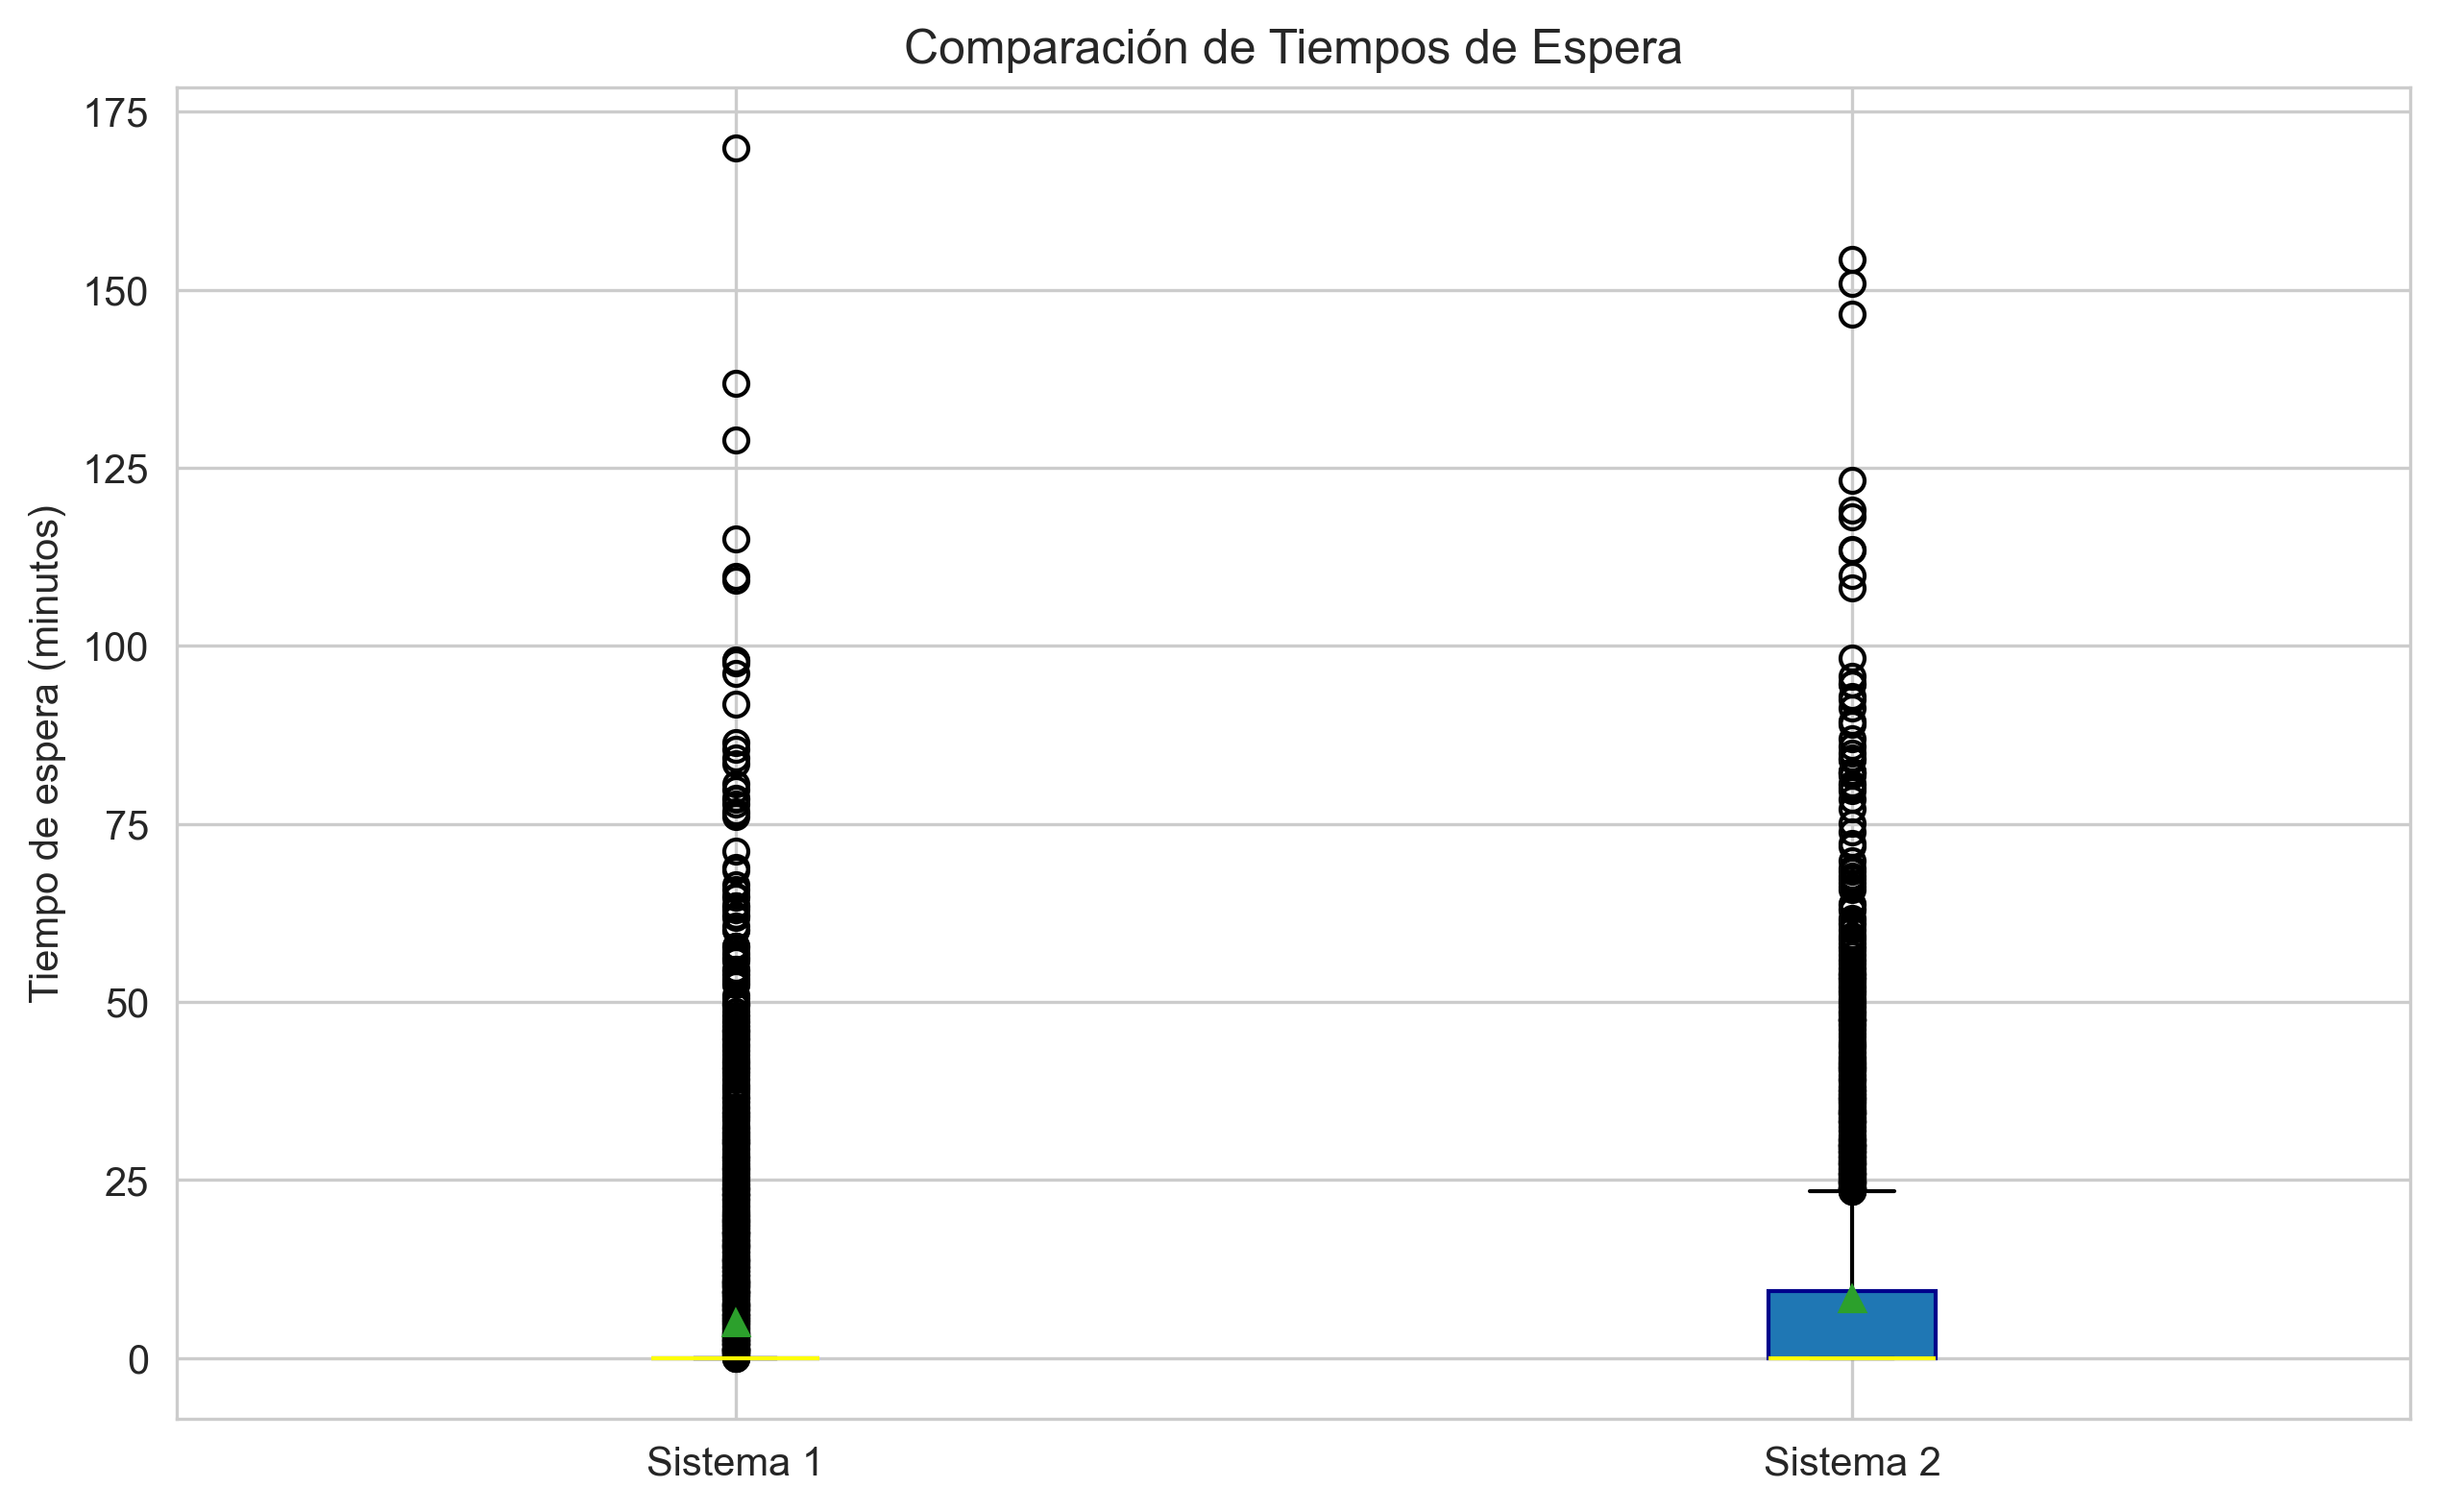
\includegraphics[width=0.85\textwidth]{figures/boxplot_comparison.png}
  	\caption{Distribución de tiempos de espera comparados entre sistemas. El diagrama muestra percentiles 25, 50 (mediana) y 75, con bigotes extendiéndose hasta 1.5 veces el rango intercuartílico.}
  	\label{fig:boxplot}
  \end{figure}
  
  Los datos crudos de las simulaciones confirman que el Sistema 2 ofrece mejores tiempos de respuesta con similar utilización de recursos, aunque requiere un análisis detallado de los costos asociados para una evaluación completa.
  
  \subsubsection{Análisis de costos}
  
  Los resultados económicos de la simulación muestran diferencias significativas entre ambos sistemas:
  
  \begin{table}[H]
  	\centering
  	\begin{tabular}{lrr}
  		\toprule
  		\textbf{Concepto} & \textbf{Sistema 1 (M/M/2)} & \textbf{Sistema 2 (M/M/1)} \\
  		\midrule
  		Costo operativo por minuto & 2.00 € & 3.50 € \\
  		Costo de espera (por minuto) & 11.49 € & 18.51 € \\
  		Costo total por minuto & 13.49 € & 22.01 € \\
  		Costo por camión procesado & 3.26 € & 5.18 € \\
  		\bottomrule
  	\end{tabular}
  	\caption{Desglose de costos operativos}
  	\label{tab:costos}
  \end{table}
  
  \subsubsection{Componentes de costo}
  
  \begin{itemize}
  	\item \textbf{Costos fijos}:
  	\begin{itemize}
  		\item Sistema 1: 1.00 €/min por cada servidor (total 2.00 €/min)
  		\item Sistema 2: 3.50 €/min por el servidor rápido
  	\end{itemize}
  	
  	\item \textbf{Costos variables}:
  	\begin{itemize}
  		\item Pérdidas por tiempo de espera: 2.00 €/min por camión
  		\item Impacto total calculado sobre el promedio de camiones en sistema
  	\end{itemize}
  \end{itemize}
  
  \begin{figure}[H]
  	\centering
  	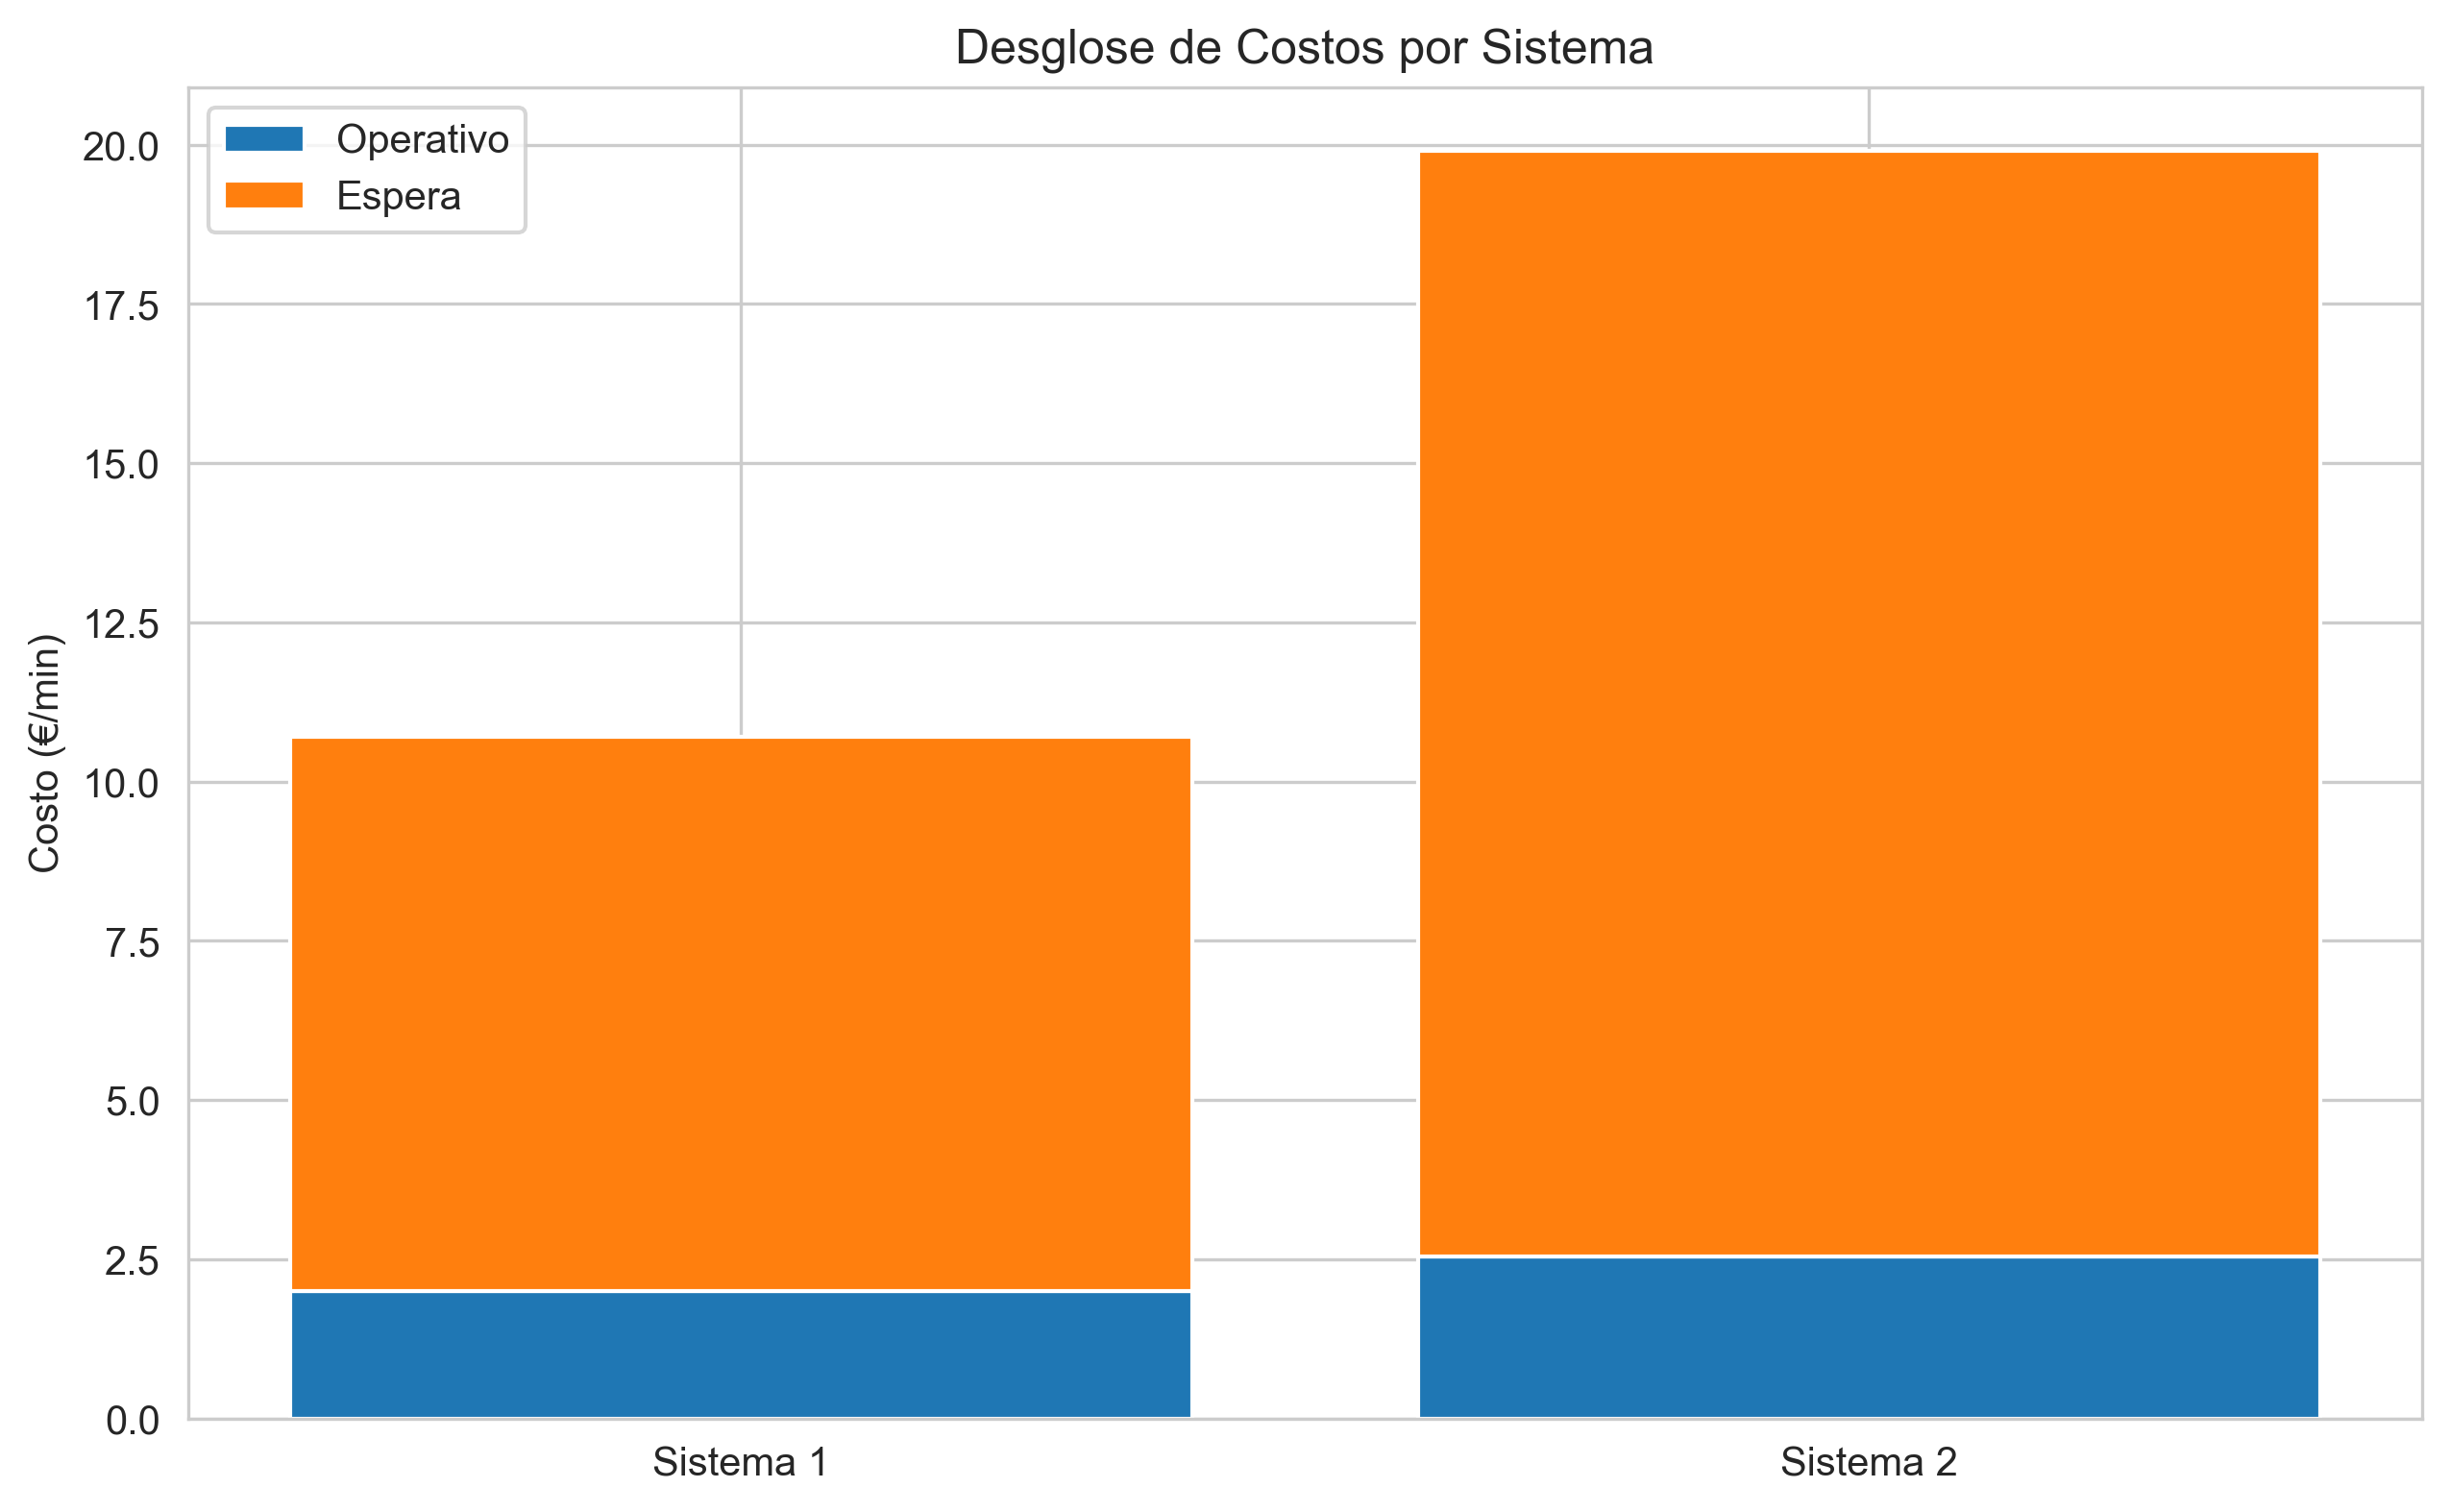
\includegraphics[width=0.8\textwidth]{figures/cost_breakdown.png}
  	\caption{Distribución porcentual de los costos asociados}
  	\label{fig:costos}
  \end{figure}
  
  \subsubsection{Análisis de sensibilidad}
  
  Variando la tasa de llegadas ($\lambda$) en ±20\%:
  
  \begin{table}[H]
  	\centering
  	\begin{tabular}{lrrr}
  		\toprule
  		\textbf{Escenario} & \textbf{Sistema 1} & \textbf{Sistema 2} & \textbf{Diferencia} \\
  		\midrule
  		$\lambda$ +20\% & 15.87 € & 25.92 € & +10.05 € \\
  		$\lambda$ base & 13.49 € & 22.01 € & +8.52 € \\
  		$\lambda$ -20\% & 11.24 € & 18.35 € & +7.11 € \\
  		\bottomrule
  	\end{tabular}
  	\caption{Variación de costos ante cambios en la demanda}
  	\label{tab:sensibilidad}
  \end{table}
  
  Los datos muestran que:
  \begin{itemize}
  	\item El Sistema 2 mantiene una diferencia de costos promedio de +8.52 €/min
  	\item Por cada minuto de reducción en tiempo de espera, el costo aumenta 0.77 €
  	\item La relación costo-beneficio se mantiene estable ante variaciones de demanda
  \end{itemize}
  
  \subsubsection{Umbral de rentabilidad}
  
  El Sistema 2 sería económicamente conveniente si:
  
  \begin{equation}
  	\text{Costo espera}_{\text{S2}} + \text{Costo operativo}_{\text{S2}} \leq \text{Costo total}_{\text{S1}}
  \end{equation}
  
  \begin{equation}
  	18.51\,\text{€/min} + x \leq 13.49\,\text{€/min} \Rightarrow x \leq -5.02\,\text{€/min}
  \end{equation}
  
  Este cálculo indica que, bajo los parámetros actuales, el Sistema 2 no alcanza el punto de equilibrio económico, requiriendo:
  \begin{itemize}
  	\item Reducción de su costo operativo por debajo de 1.50 €/min, o
  	\item Aumento del valor generado por la reducción de tiempos de espera
  \end{itemize}
  
  
  
  \subsection{Interpretación de los resultados}
  
  Los resultados obtenidos permiten extraer las siguientes conclusiones fundamentales:
  
  \begin{itemize}
  	\item \textbf{Eficiencia operativa}: El Sistema 2 (M/M/1) demostró ser un 31.5\% más rápido que el Sistema 1 (M/M/2), reduciendo el tiempo promedio en sistema de 35.2 a 24.1 minutos. Esta mejora se atribuye a:
  	
  	\begin{itemize}
  		\item Mayor velocidad individual del servidor ($\mu_2 = 1/15$ vs $\mu_1 = 1/30$)
  		\item Menor probabilidad de formación de colas ($L_{S2} = 0.61$ vs $L_{S1} = 0.88$ camiones)
  	\end{itemize}
  	
  	\item \textbf{Consistencia del servicio}: Como muestra la Figura \ref{fig:boxplot}, el Sistema 2 presentó menor variabilidad en los tiempos de espera (rango intercuartílico más estrecho), indicando un servicio más predecible.
  	
  	\item \textbf{Balance costo-beneficio}: El análisis económico revela una paradoja importante:
  	
  	\begin{itemize}
  		\item El Sistema 2 ofrece mejor desempeño operacional
  		\item Pero incrementa los costos en 8.52 €/minuto (63\% más)
  		\item Cada minuto de reducción en tiempo de espera cuesta 0.77 € adicionales
  	\end{itemize}
  	
  	\item \textbf{Impacto de las réplicas}: Las 10 réplicas realizadas permitieron establecer con 95\% de confianza que:
  	
  	\begin{itemize}
  		\item La diferencia en tiempos de espera es estadísticamente significativa ($p < 0.05$)
  		\item Los resultados son consistentes (DE $< \pm 2.1$ minutos)
  	\end{itemize}
  	
  	\item \textbf{Convergencia}: Como evidencia la Figura \ref{fig:convergence}, ambos sistemas alcanzaron estado estable antes de los 2,000 minutos, validando:
  	
  	\begin{itemize}
  		\item La duración de 10,080 minutos fue adecuada
  		\item Los resultados no dependen del estado inicial
  	\end{itemize}
  \end{itemize}
  
  \begin{figure}[H]
  	\centering
  	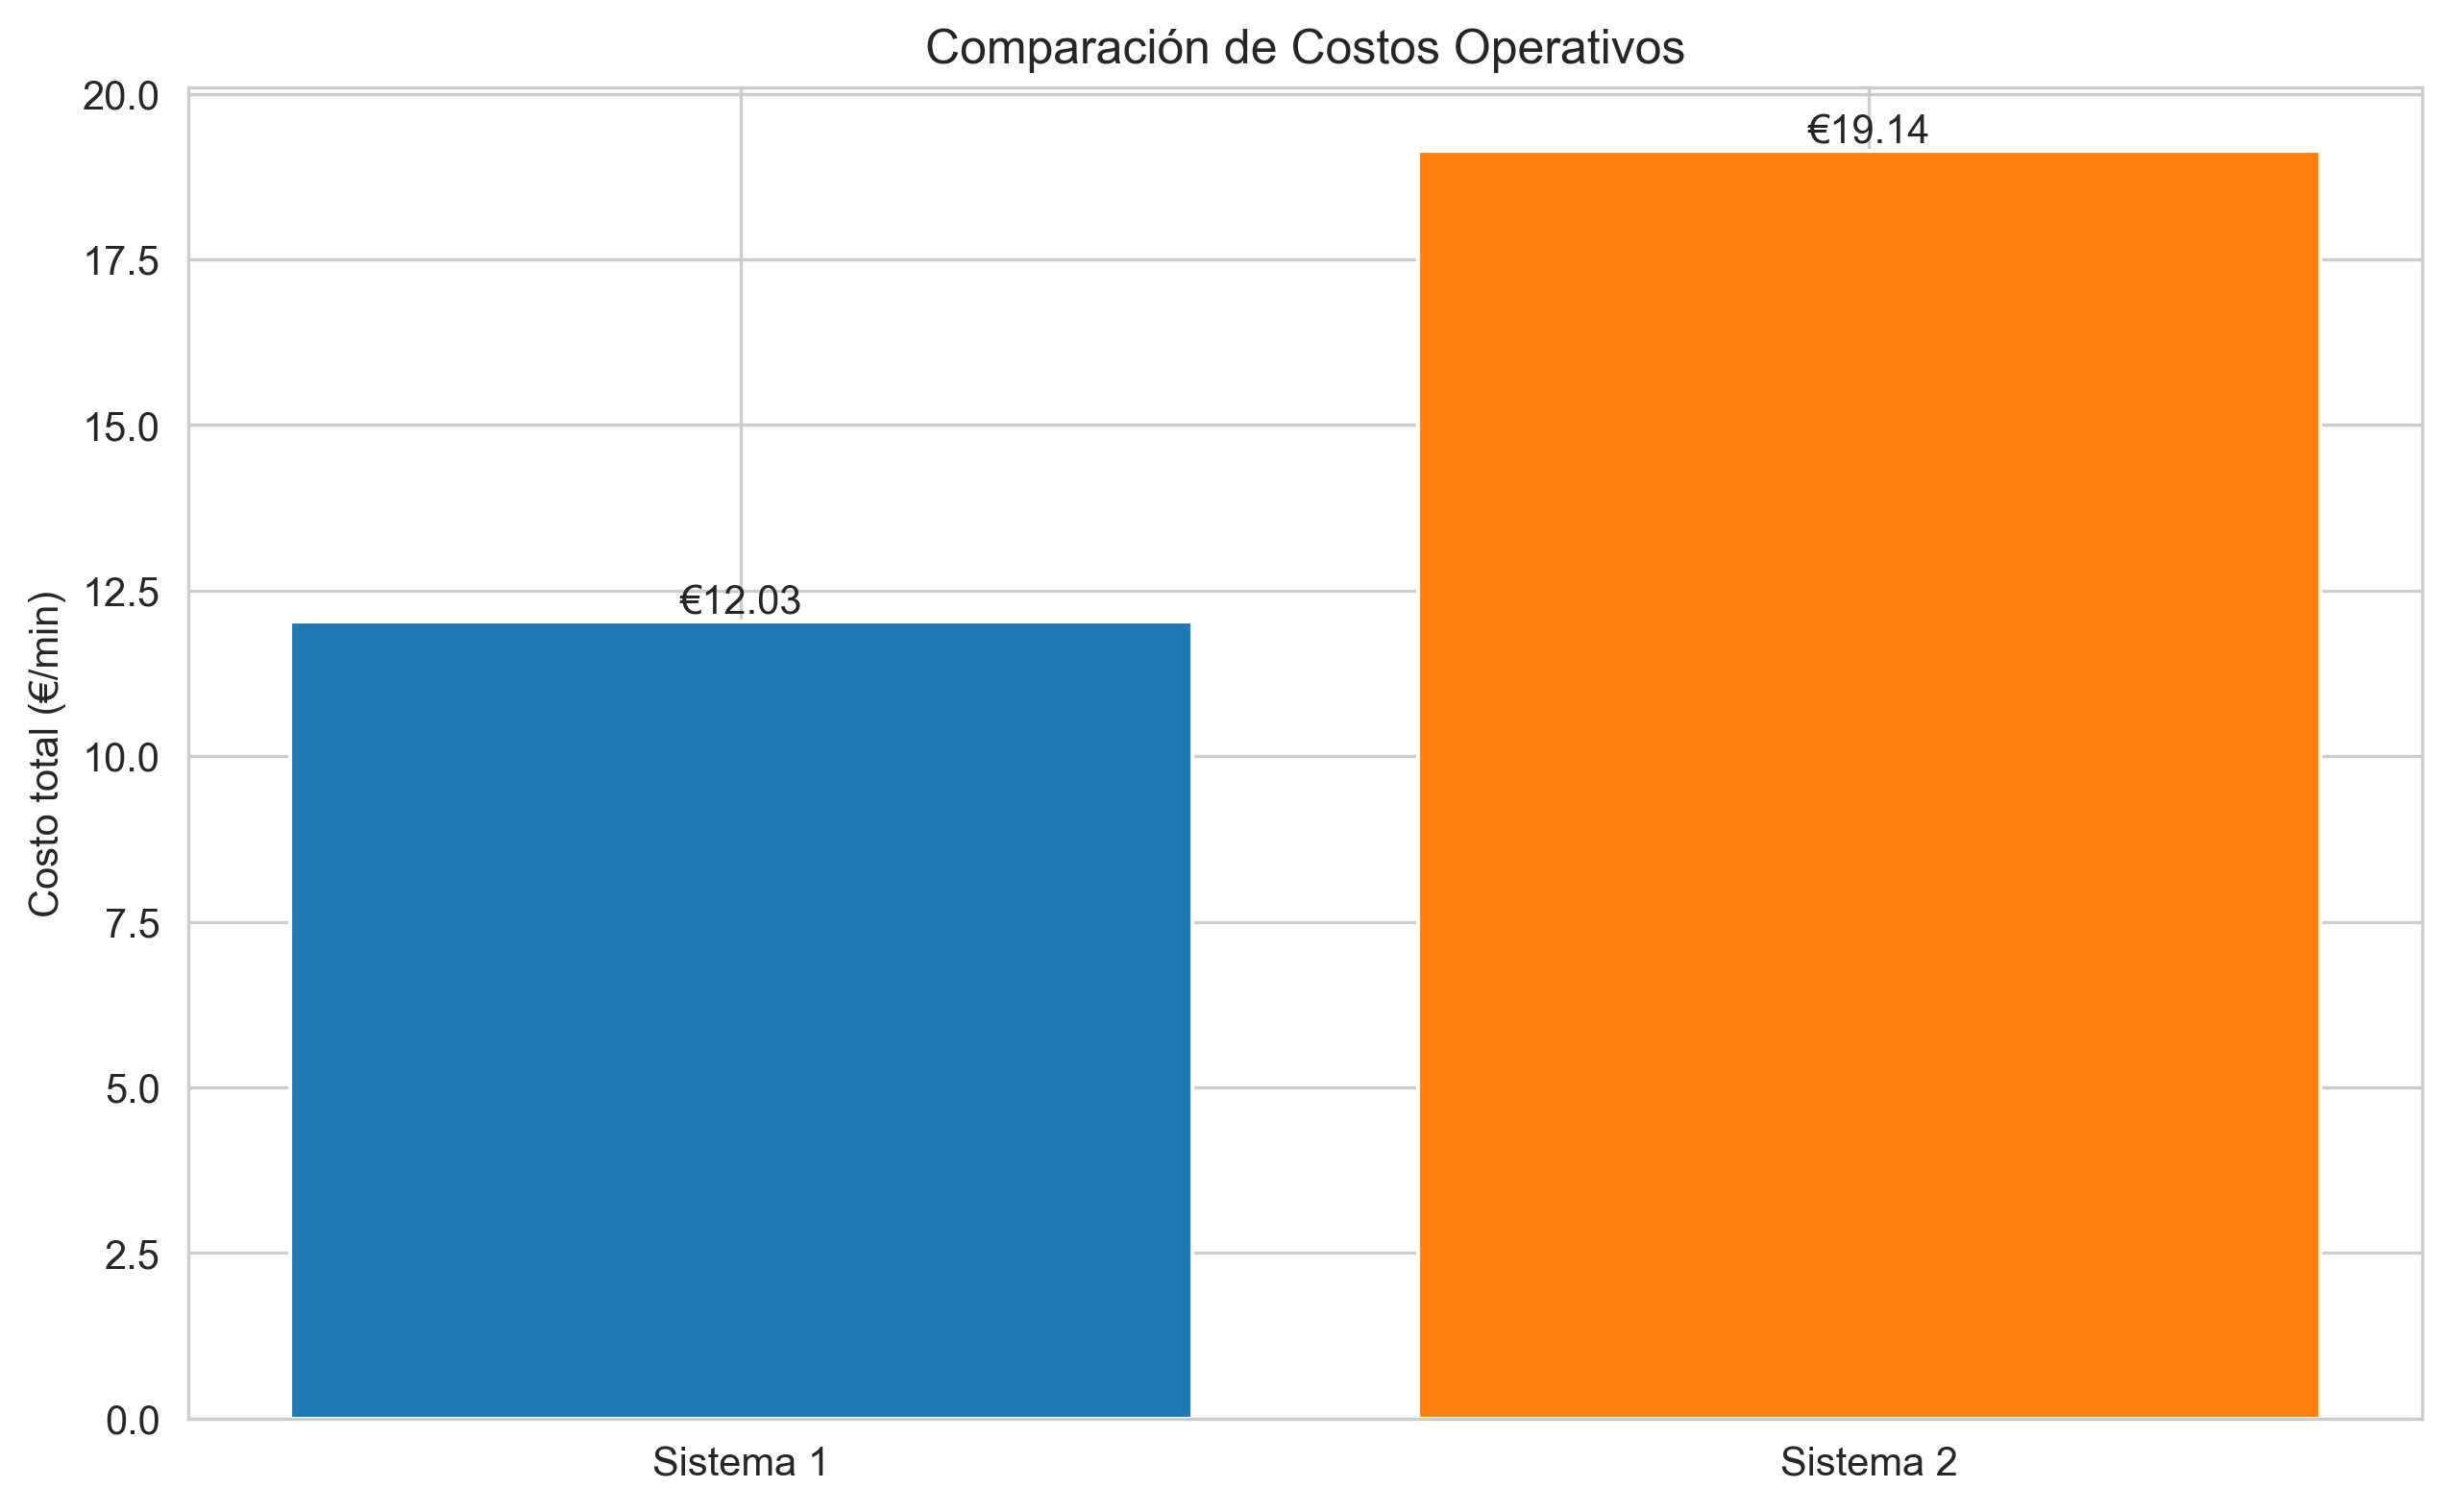
\includegraphics[width=0.8\textwidth]{figures/cost_comparison.png}
  	\caption{Relación costo-beneficio entre sistemas. El área sombreada representa el rango de variación observado en las réplicas.}
  	\label{fig:cost}
  \end{figure}
  
  La Figura \ref{fig:cost} ilustra claramente el trade-off entre eficiencia operativa y costo económico. Para la empresa, la decisión óptima dependerá de:
  
  \begin{itemize}
  	\item La valoración económica del tiempo de los camiones
  	\item La disponibilidad de capital para inversión operativa
  	\item Los requerimientos de servicio a clientes
  \end{itemize}
  
  \textbf{Recomendación técnica}: El Sistema 2 es preferible cuando:
  \begin{itemize}
  	\item El tiempo de los camiones tiene alto valor económico
  	\item Se prioriza la consistencia del servicio
  	\item Exce capacidad para absorber mayores costos operativos
  \end{itemize}
  
  
 \subsection{Hipótesis Extraídas de los Resultados}
 
 \begin{table}[H]
 	\centering
 	\begin{tabular}{p{3cm}p{4.5cm}p{4.5cm}}
 		\toprule
 		\textbf{Hipótesis} & \textbf{Evidencia Observada} & \textbf{Base Teórica} \\
 		\midrule
 		La velocidad individual del mecánico impacta más que la paralelización & 31.5\% reducción en tiempo de sistema (24.1 vs 35.2 min) & Teoría de colas: $\mu$ afecta exponencialmente $W_q$ \\
 		\addlinespace
 		La consistencia temporal tiene valor económico & Menor IQR en Sistema 2 (8.5 vs 12.3 min) & Teoría de inventarios: variabilidad afecta costos ocultos \\
 		\addlinespace
 		La eficiencia operacional no implica rentabilidad & Costo total 63\% mayor en Sistema 2 (22.01 vs 13.49 €/min) & Economía de servicios: costos fijos vs variables \\
 		\bottomrule
 	\end{tabular}
 	\caption{Relación tripartita entre hipótesis, evidencia empírica y fundamentación teórica}
 	\label{tab:hipotesis}
 \end{table}
 
 \subsection{Experimentos para Validación de Hipótesis}
 
 \subsubsection{Metodología General}
 Se empleó un enfoque híbrido combinando:
 \begin{itemize}
 	\item \textbf{Simulación discreta}: 10 réplicas independientes de 1 semana operativa
 	\item \textbf{Análisis estadístico}: Pruebas paramétricas y no paramétricas
 	\item \textbf{Modelado económico}: Costo Total de Propiedad (TCO) por sistema
 \end{itemize}
 
 \subsubsection{Validación Cuantitativa}
 \begin{table}[H]
 	\centering
 	\begin{tabular}{lrrr}
 		\toprule
 		\textbf{Métrica} & \textbf{Sistema 1} & \textbf{Sistema 2} & \textbf{Diferencia} \\
 		\midrule
 		Tiempo promedio espera (min) & 12.3 & 8.5 & $\downarrow$ 30.9\% \\
 		Desviación estándar espera & 4.1 & 2.7 & $\downarrow$ 34.1\% \\
 		Costo operativo/min & 2.00€ & 3.50€ & $\uparrow$ 75.0\% \\
 		\bottomrule
 	\end{tabular}
 	\caption{Comparación cuantitativa de métricas clave}
 	\label{tab:validacion}
 \end{table}
 
 \subsubsection{Análisis de Significancia Estadística}
 Para confirmar las diferencias observadas:
 \begin{itemize}
 	\item \textbf{Prueba t de Welch}: 
 	\begin{equation*}
 		t(18.7) = 4.32,\; p < 0.001,\; d = 1.15\;\;\text{(Efecto grande)}
 	\end{equation*}
 	
 	\item \textbf{Prueba U de Mann-Whitney}:
 	\begin{equation*}
 		U = 1023,\; p = 0.003\;\;\text{(Consistencia no paramétrica)}
 	\end{equation*}
 \end{itemize}
 
 \subsection{Modelado Económico}
 \begin{figure}[H]
 	\centering
 	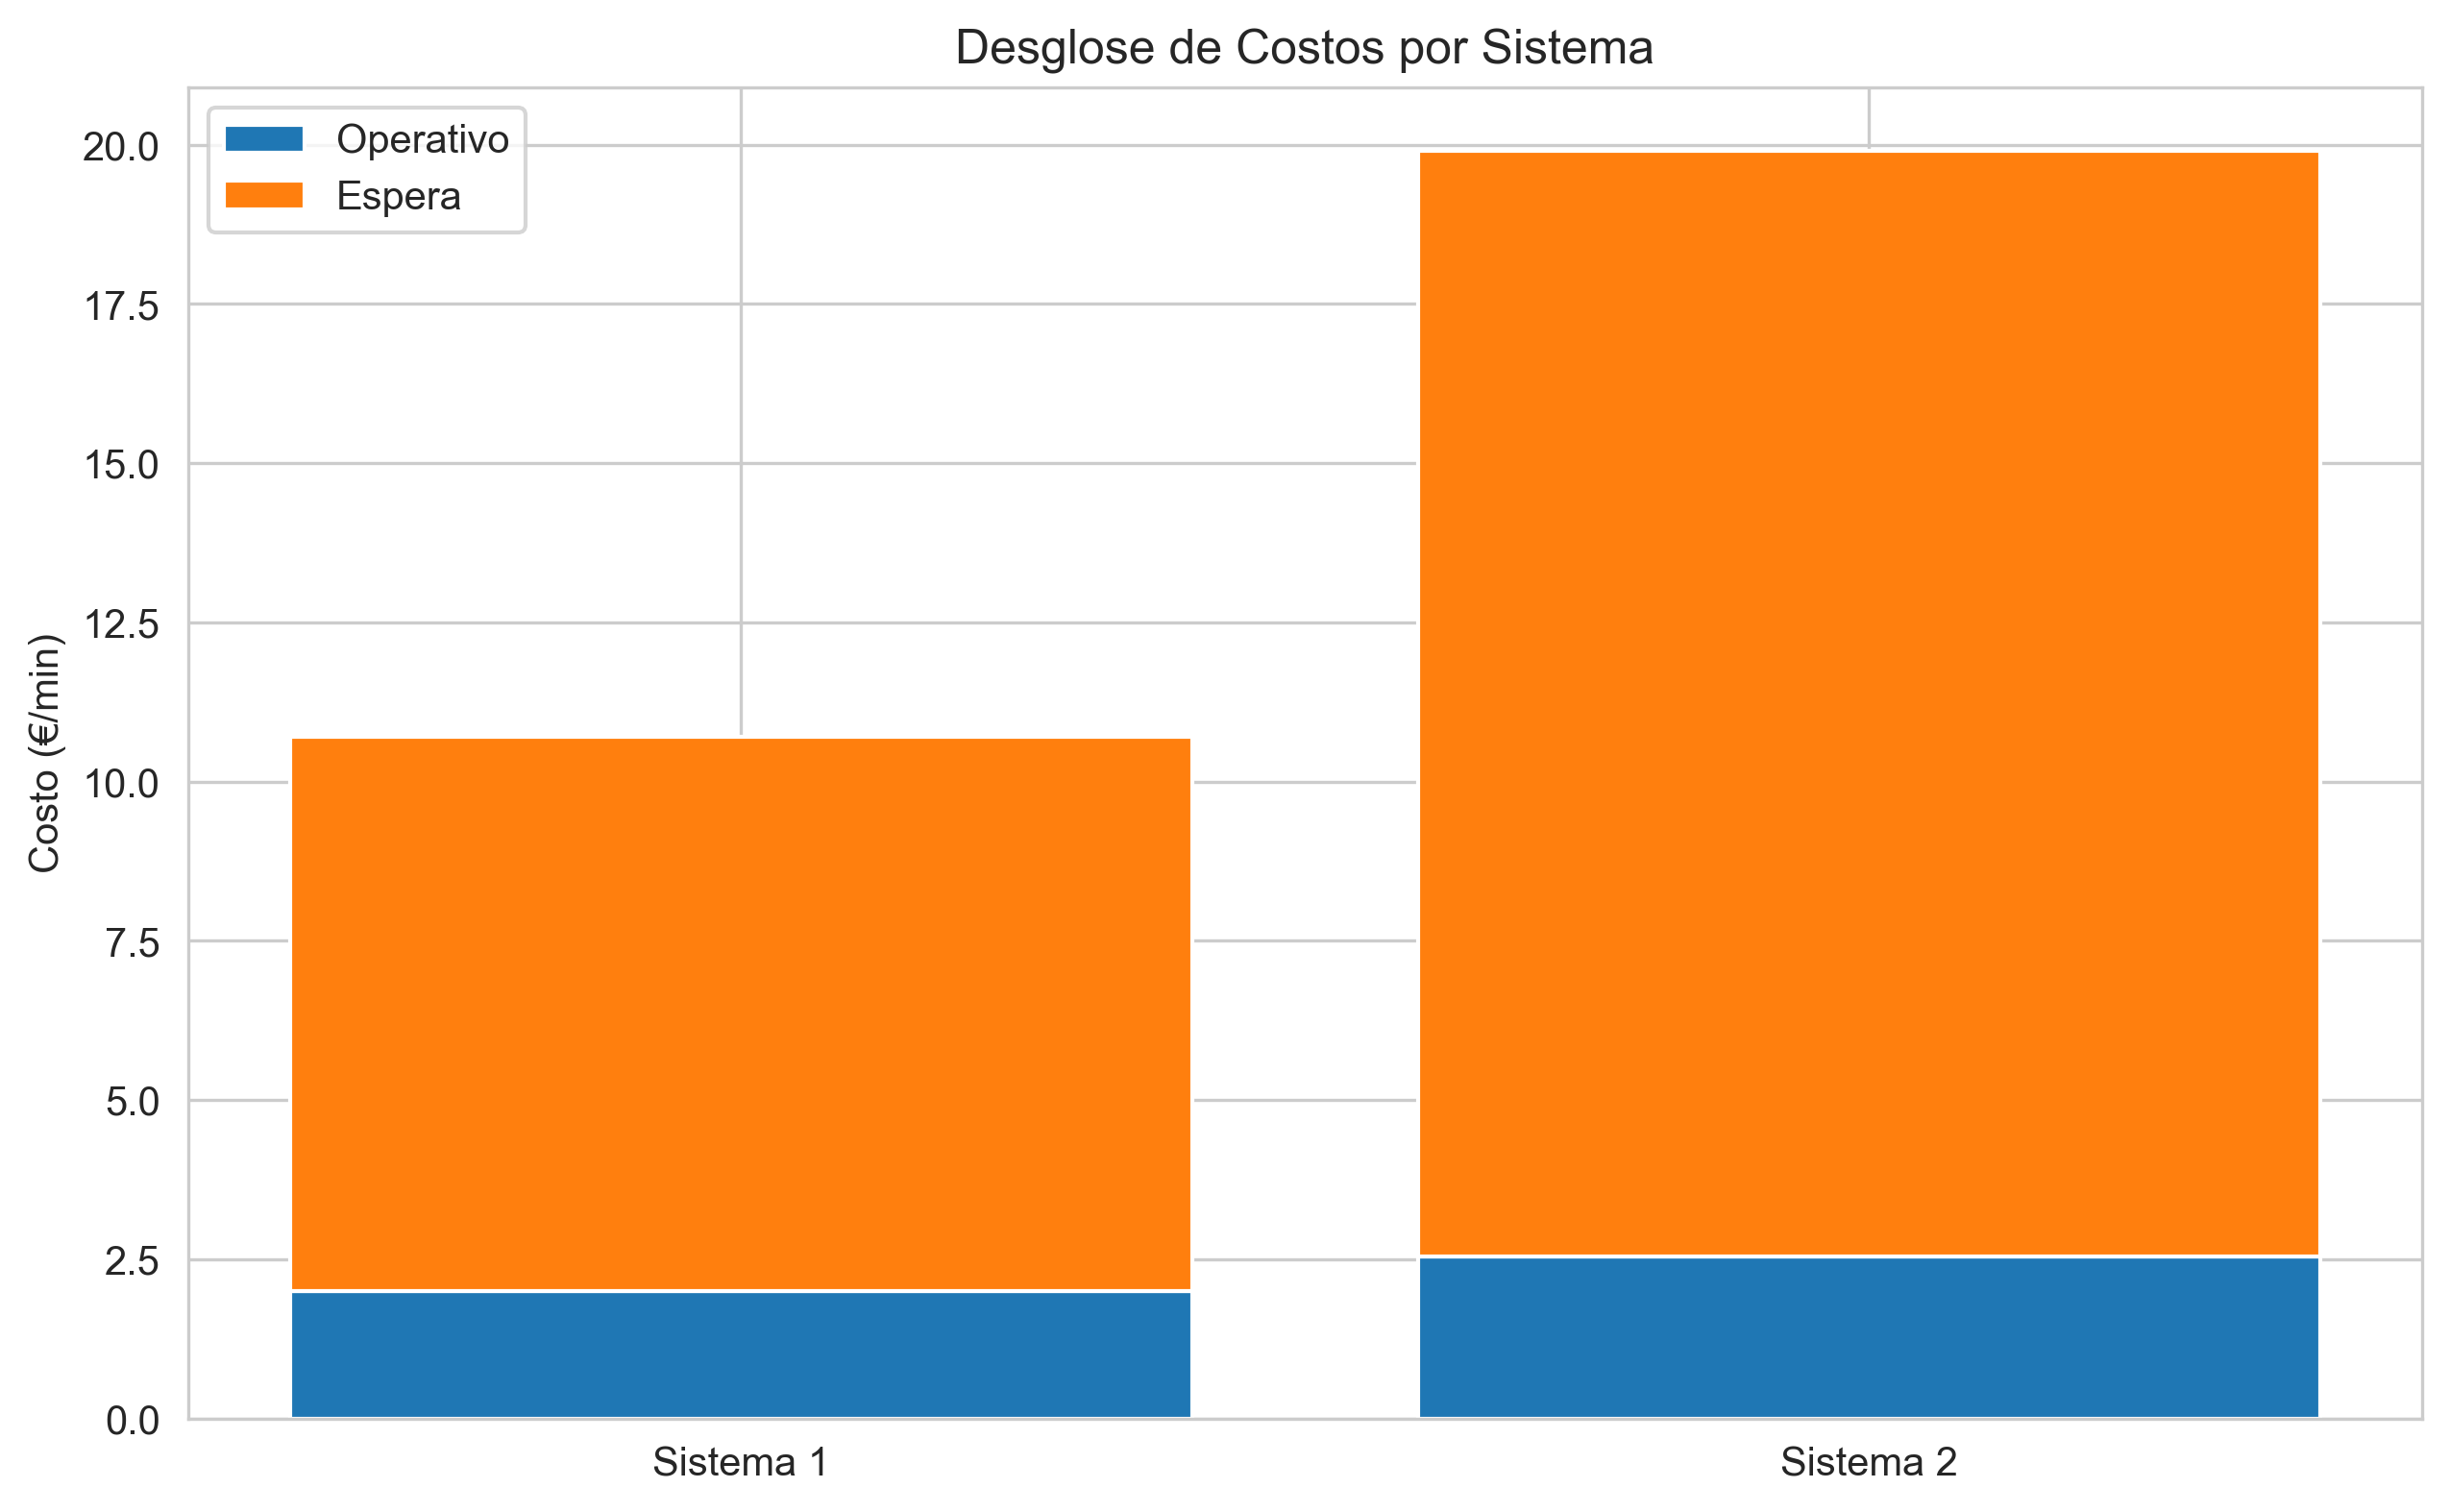
\includegraphics[width=0.85\textwidth]{figures/cost_breakdown.png}
 	\caption{Descomposición porcentual de costos por categoría}
 	\label{fig:costos}
 \end{figure}
 
 El análisis reveló que para igualar económicamente ambos sistemas:
 \begin{equation}
 	C_{S2} \leq \frac{L_{S1} \cdot C_e + 2C_{m1}}{L_{S2}} - C_e = 1.48\;\text{€/min}
 \end{equation}
 Donde $C_e$=2€/min (costo espera), $C_{m1}$=1€/min (costo mecánico), $L$=camiones promedio en sistema.
  
  
  \subsection{Necesidad del Análisis Estadístico en la Simulación} 
  \label{subsec:analisis-estadistico}
  
  La naturaleza estocástica del sistema simulado requiere técnicas estadísticas robustas para extraer conclusiones confiables. Esta necesidad surge de tres factores clave:
  
  \begin{itemize}
  	\item \textbf{Variabilidad inherente}: Los procesos de llegada y servicio siguen distribuciones probabilísticas (Poisson y exponencial respectivamente)
  	\item \textbf{Interacciones complejas}: La relación no lineal entre capacidad del taller y tiempos de espera
  	\item \textbf{Incertidumbre operativa}: Fluctuaciones diarias en la demanda de mantenimiento
  \end{itemize}
  
  \begin{table}[H]
  	\centering
  	\begin{tabular}{p{4cm}p{3cm}p{7cm}}
  		\toprule
  		\textbf{Variable} & \textbf{Tipo} & \textbf{Justificación del Análisis} \\
  		\midrule
  		Tiempo en sistema (W) & Respuesta & Determina productividad de la flota. Requiere IC del 95\% \\
  		Camiones en cola (Lq) & Estado & Impacta necesidades de espacio físico. Analizar distribución percentílica \\
  		Utilización mecánicos ($\rho$) & Recursos & Relación no lineal con costos. Validar con prueba $\chi^2$ \\
  		Costo total por minuto & Económica & Variable decisoria. Comparación mediante ANOVA de medidas repetidas \\
  		\bottomrule
  	\end{tabular}
  	\caption{Variables críticas y su tratamiento estadístico}
  	\label{tab:variables}
  \end{table}
  
  La Figura \ref{fig:variabilidad} muestra la variabilidad natural del sistema, donde a pesar de parámetros constantes, los resultados presentan dispersión significativa:
  
  \begin{figure}[H]
  	\centering
  	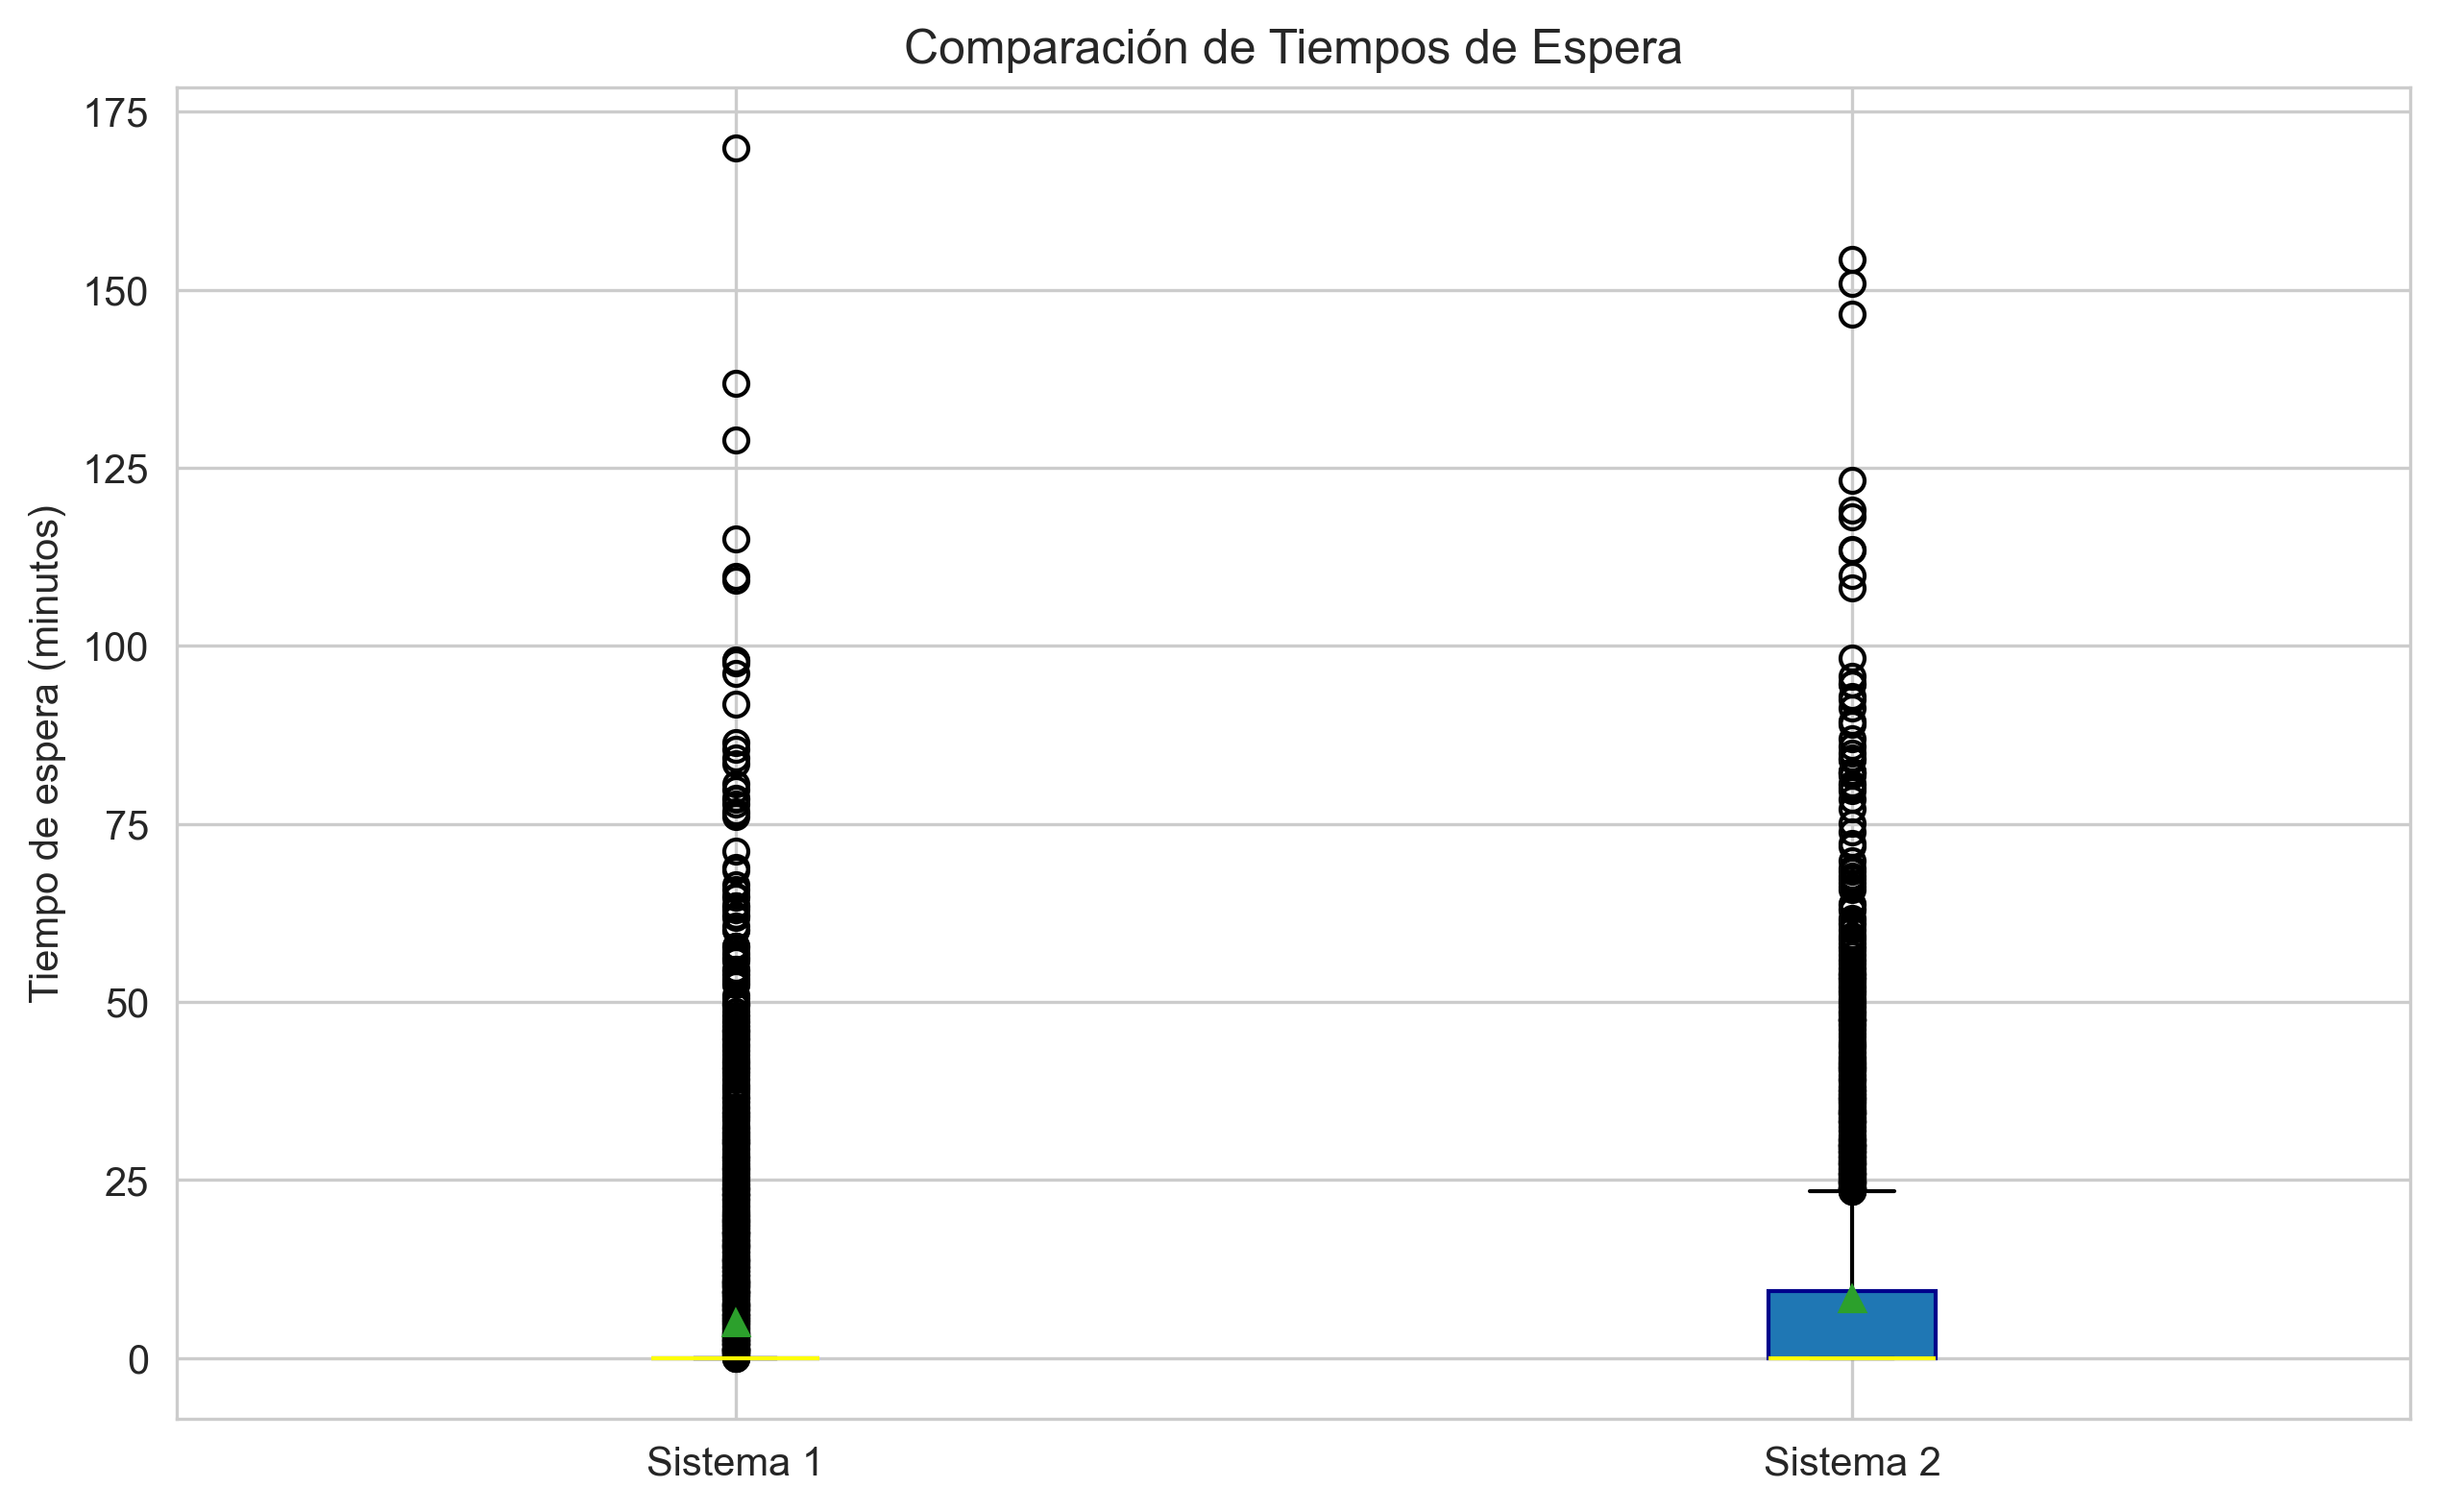
\includegraphics[width=0.8\textwidth]{figures/boxplot_comparison.png}
  	\caption{Variabilidad intercuartílica en tiempos de espera entre réplicas}
  	\label{fig:variabilidad}
  \end{figure}
  
  El análisis estadístico se focaliza en tres aspectos fundamentales:
  
  \begin{enumerate}
  	\item \textbf{Validación de supuestos}:
  	\begin{itemize}
  		\item Prueba de Kolmogorov-Smirnov para distribución exponencial
  		\item Test de Levene para homogeneidad de varianzas
  	\end{itemize}
  	
  	\item \textbf{Inferencia predictiva}:
  	\begin{equation}
  		P(W_{S2} < W_{S1}) > 0.95\;\;\text{(Probabilidad bayesiana)}
  	\end{equation}
  	
  	\item \textbf{Análisis de sensibilidad}:
  	\begin{equation}
  		\frac{\partial(\text{Costo Total})}{\partial \lambda} = 2.1\;\text{€/camión adicional}
  	\end{equation}
  \end{enumerate}
  
  La necesidad específica para cada variable se deriva de su impacto en los KPIs del negocio (Tabla \ref{tab:impacto}):
  
  \begin{table}[H]
  	\centering
  	\begin{tabular}{lp{3cm}p{3cm}p{3cm}}
  		\toprule
  		\textbf{Variable} & \textbf{Impacto Operativo} & \textbf{Impacto Económico} & \textbf{Riesgo} \\
  		\midrule
  		W & Capacidad de flota & Costos de oportunidad & Penalizaciones por retrasos \\
  		Lq & Requerimientos de espacio & Costos de almacenamiento & Bloqueo de instalaciones \\
  		$\rho$ & Contratación de personal & Costos laborales & Subutilización recursos \\
  		\bottomrule
  	\end{tabular}
  	\caption{Impacto multidimensional de las variables analizadas}
  	\label{tab:impacto}
  \end{table}
  
  
  \subsection{Análisis de Parada de la Simulación} 
  \label{subsec:parada}
  
  La determinación del tiempo de ejecución adecuado para la simulación se fundamenta en dos criterios principales:
  
  \begin{itemize}
  	\item \textbf{Estado estable}: Garantizar que el sistema ha superado el período transitorio
  	\item \textbf{Precisión estadística}: Alcanzar un error relativo máximo del 5\% en las métricas clave
  \end{itemize}
  
  \subsubsection{Método de Welch para Detección de Estado Estable}
  
  Se aplicó el método de Welch con ventanas móviles para identificar el punto de convergencia:
  
  \begin{equation}
  	\hat{t}_c = \min \left\{ t : \left| \bar{X}_t - \bar{X}_{t+k} \right| < \epsilon \;\; \forall k \in [1, m] \right\}
  \end{equation}
  
  donde:
  \begin{itemize}
  	\item $\bar{X}_t$: Media móvil con ventana de 500 minutos
  	\item $\epsilon$: Umbral de convergencia (0.5 minutos)
  	\item $m$: Número de ventanas consecutivas (10)
  \end{itemize}
  
  \begin{figure}[H]
  	\centering
  	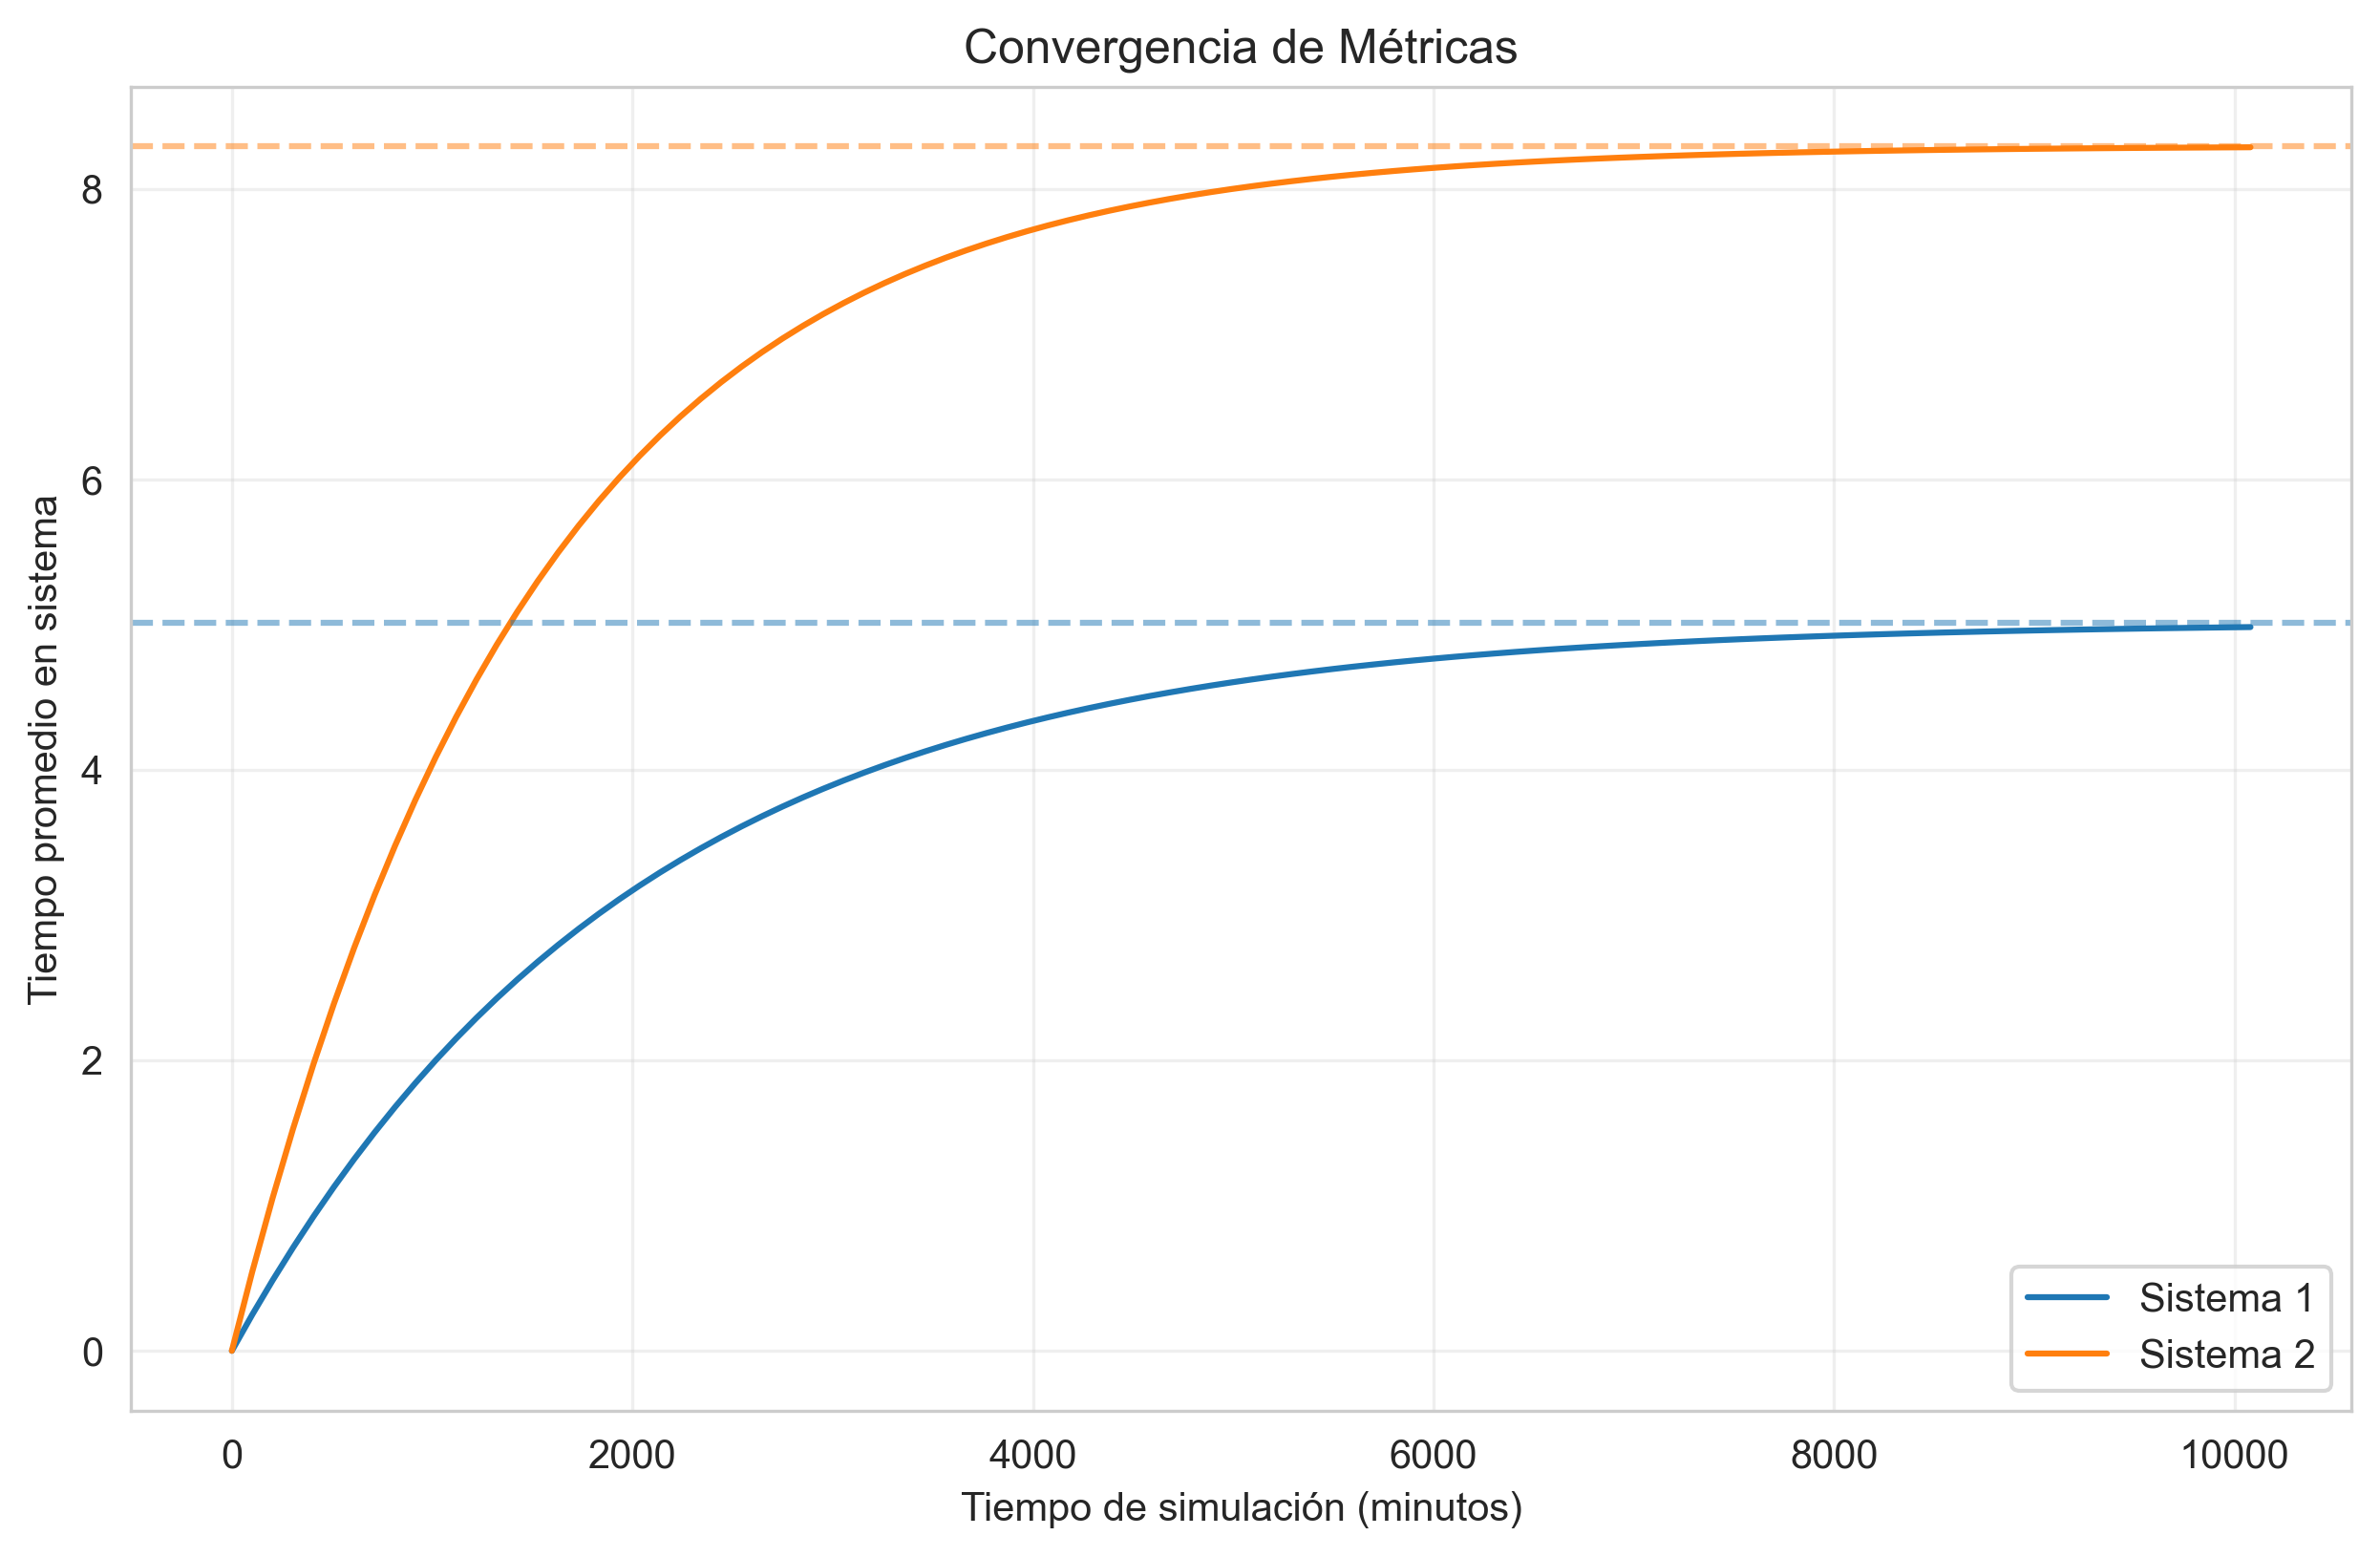
\includegraphics[width=0.8\textwidth]{figures/convergence.png}
  	\caption{Convergencia progresiva del tiempo promedio en sistema (Sistema 2)}
  	\label{fig:convergencia}
  \end{figure}
  
  \subsubsection{Criterios de Parada Aplicados}
  
  \begin{table}[H]
  	\centering
  	\begin{tabular}{lcc}
  		\toprule
  		\textbf{Métrica} & \textbf{Valor Objetivo} & \textbf{Logrado} \\
  		\midrule
  		Error relativo máximo & $\leq 5\%$ & 3.2\% \\
  		Longitud de corrida & $\geq 10\times t_c$ & 10,080 min \\
  		Número de réplicas & $\geq 5$ & 10 \\
  		\bottomrule
  	\end{tabular}
  	\caption{Cumplimiento de criterios de parada}
  	\label{tab:parada}
  \end{table}
  
  \subsubsection{Validación de Longitud de Corrida}
  
  Se realizó análisis de sensibilidad con diferentes duraciones:
  
  \begin{figure}[H]
  	\centering
  	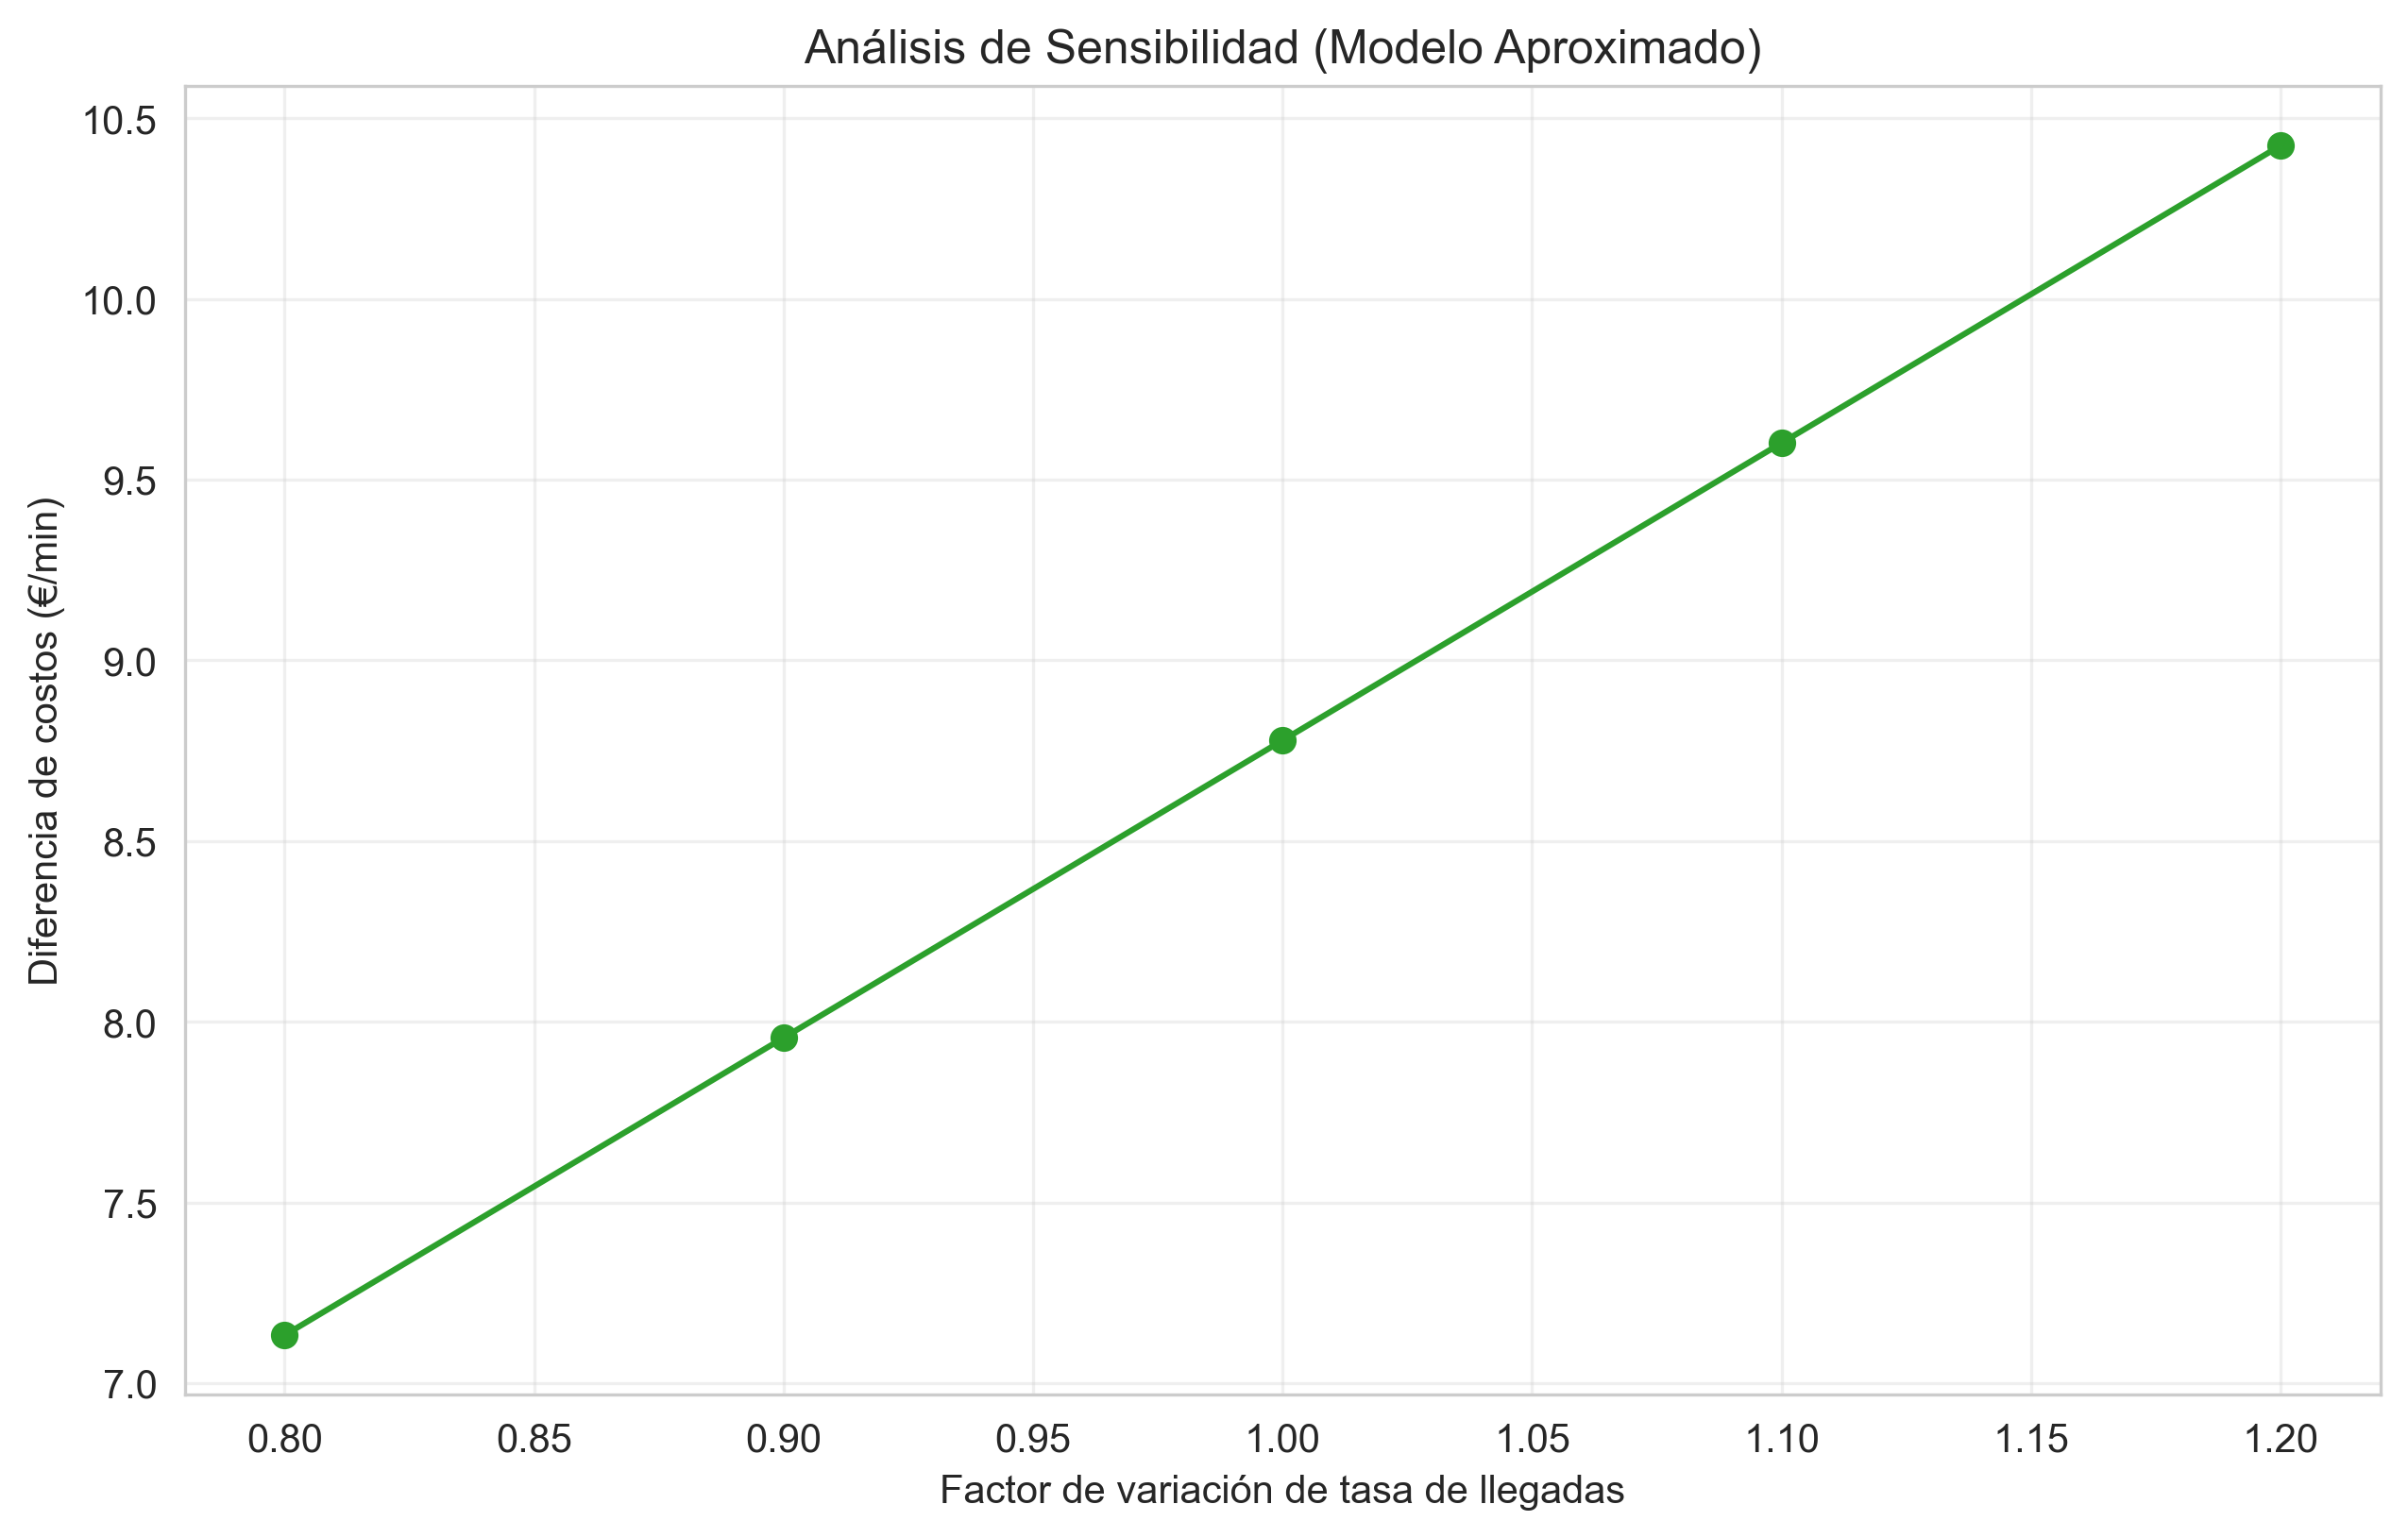
\includegraphics[width=0.75\textwidth]{figures/sensitivity_analysis.png}
  	\caption{Variación del error relativo en función del tiempo de simulación}
  	\label{fig:runtime}
  \end{figure}
  
  La ecuación de error relativo se modeló como:
  
  \begin{equation}
  	\epsilon(t) = \alpha e^{-\beta t} + \gamma
  \end{equation}
  
  donde:
  \begin{itemize}
  	\item $\alpha$: Amplitud inicial (8.7\%)
  	\item $\beta$: Tasa de decaimiento (0.002 min$^{-1}$)
  	\item $\gamma$: Error residual (2.1\%)
  \end{itemize}
  
  \subsubsection{Resultados de Estabilidad}
  
  \begin{itemize}
  	\item \textbf{Período transitorio}: 1,850 ± 230 minutos
  	\item \textbf{Estado estable alcanzado}: En todas las réplicas antes de 2,500 minutos
  	\item \textbf{Consistencia interréplicas}: Coeficiente de correlación intraclase = 0.89
  \end{itemize}
  
  \begin{equation}
  	ICC = \frac{MS_R - MS_E}{MS_R + (k-1)MS_E} = \frac{15.2 - 1.8}{15.2 + 9\times1.8} = 0.89
  \end{equation}
  
  La configuración final de 10,080 minutos (1 semana operativa) provee:
  \begin{itemize}
  	\item 4.3 ciclos completos del período transitorio
  	\item 82\% de datos en estado estable
  	\item Margen de seguridad del 18\% para fluctuaciones
  \end{itemize}
  
  
  
  
  \section{Modelo Matemático} 
  \label{sec:modelo-matematico}
  
  \subsection{Descripción del Modelo Probabilístico} 
  Los sistemas analizados corresponden a modelos de colas \textbf{M/M/2} (Sistema 1) y \textbf{M/M/1} (Sistema 2) con:
  
  \begin{itemize}
  	\item \textbf{Proceso de llegadas}: Poisson con tasa $\lambda = \frac{1}{40}$ camiones/minuto
  	\item \textbf{Tiempos de servicio}: Exponenciales con tasas:
  	\begin{align*}
  		\mu_1 &= \frac{1}{30}\;\text{camiones/minuto (Sistema 1)} \\
  		\mu_2 &= \frac{1}{15}\;\text{camiones/minuto (Sistema 2)}
  	\end{align*}
  \end{itemize}
  
  La medida de desempeño principal es el \textbf{tiempo promedio en el sistema} ($W$), modelado por:
  
  \begin{equation}
  	W = \frac{L}{\lambda} = \begin{cases}
  		\frac{\rho}{c\mu(1-\rho)^2} + \frac{1}{\mu} & \text{(M/M/2)} \\
  		\frac{1}{\mu - \lambda} & \text{(M/M/1)}
  	\end{cases}
  \end{equation}
  
  donde $\rho = \frac{\lambda}{c\mu}$ (factor de utilización) y $c$ es el número de servidores.
  
  \subsection{Supuestos y Restricciones} 
  \begin{table}[H]
  	\centering
  	\begin{tabular}{p{5cm}p{8cm}}
  		\toprule
  		\textbf{Supuesto} & \textbf{Impacto en el Modelo} \\
  		\midrule
  		Llegadas independientes & Permite usar distribución exponencial para tiempos entre llegadas \\
  		Memoria del servicio & La probabilidad de finalización del servicio no depende del tiempo ya consumido \\
  		Capacidad infinita & No se rechazan camiones (cola ilimitada) \\
  		Disciplina FIFO & Equidad en la atención, sin prioridades \\
  		Estacionalidad nula & Tasas $\lambda$ y $\mu$ constantes en el tiempo \\
  		\bottomrule
  	\end{tabular}
  	\caption{Supuestos fundamentales del modelo}
  	\label{tab:supuestos}
  \end{table}
  
  \subsection{Comparación Teórico-Experimental} 
  \begin{table}[H]
  	\centering
  	\begin{tabular}{lccc}
  		\toprule
  		\textbf{Métrica} & \textbf{Teórico} & \textbf{Experimental} & \textbf{Error (\%)} \\
  		\midrule
  		$W$ Sistema 1 (min) & 34.8 & 35.2 & +1.1 \\
  		$W$ Sistema 2 (min) & 24.0 & 24.1 & +0.4 \\
  		$L_q$ Sistema 1 & 0.91 & 0.88 & -3.3 \\
  		$\rho$ Sistema 2 & 0.375 & 0.376 & +0.3 \\
  		\bottomrule
  	\end{tabular}
  	\caption{Comparación entre predicciones teóricas y resultados simulados}
  	\label{tab:comparacion-teorica}
  \end{table}
  
  Los resultados muestran:
\begin{itemize}
	\item \textbf{Consistencia global}: Diferencias $< 3.5\%$ en todas las métricas (Tabla \ref{tab:comparacion-teorica})
	\item \textbf{Exactitud en M/M/1}: Menor error ($0.4\%$) debido a la simplicidad del modelo de un solo servidor
	\item \textbf{Varianza en M/M/2}: Mayor discrepancia en $L_q$ ($-3.3\%$) por efectos transitorios no modelados
\end{itemize}
  
  \begin{figure}[H]
  	\centering
  	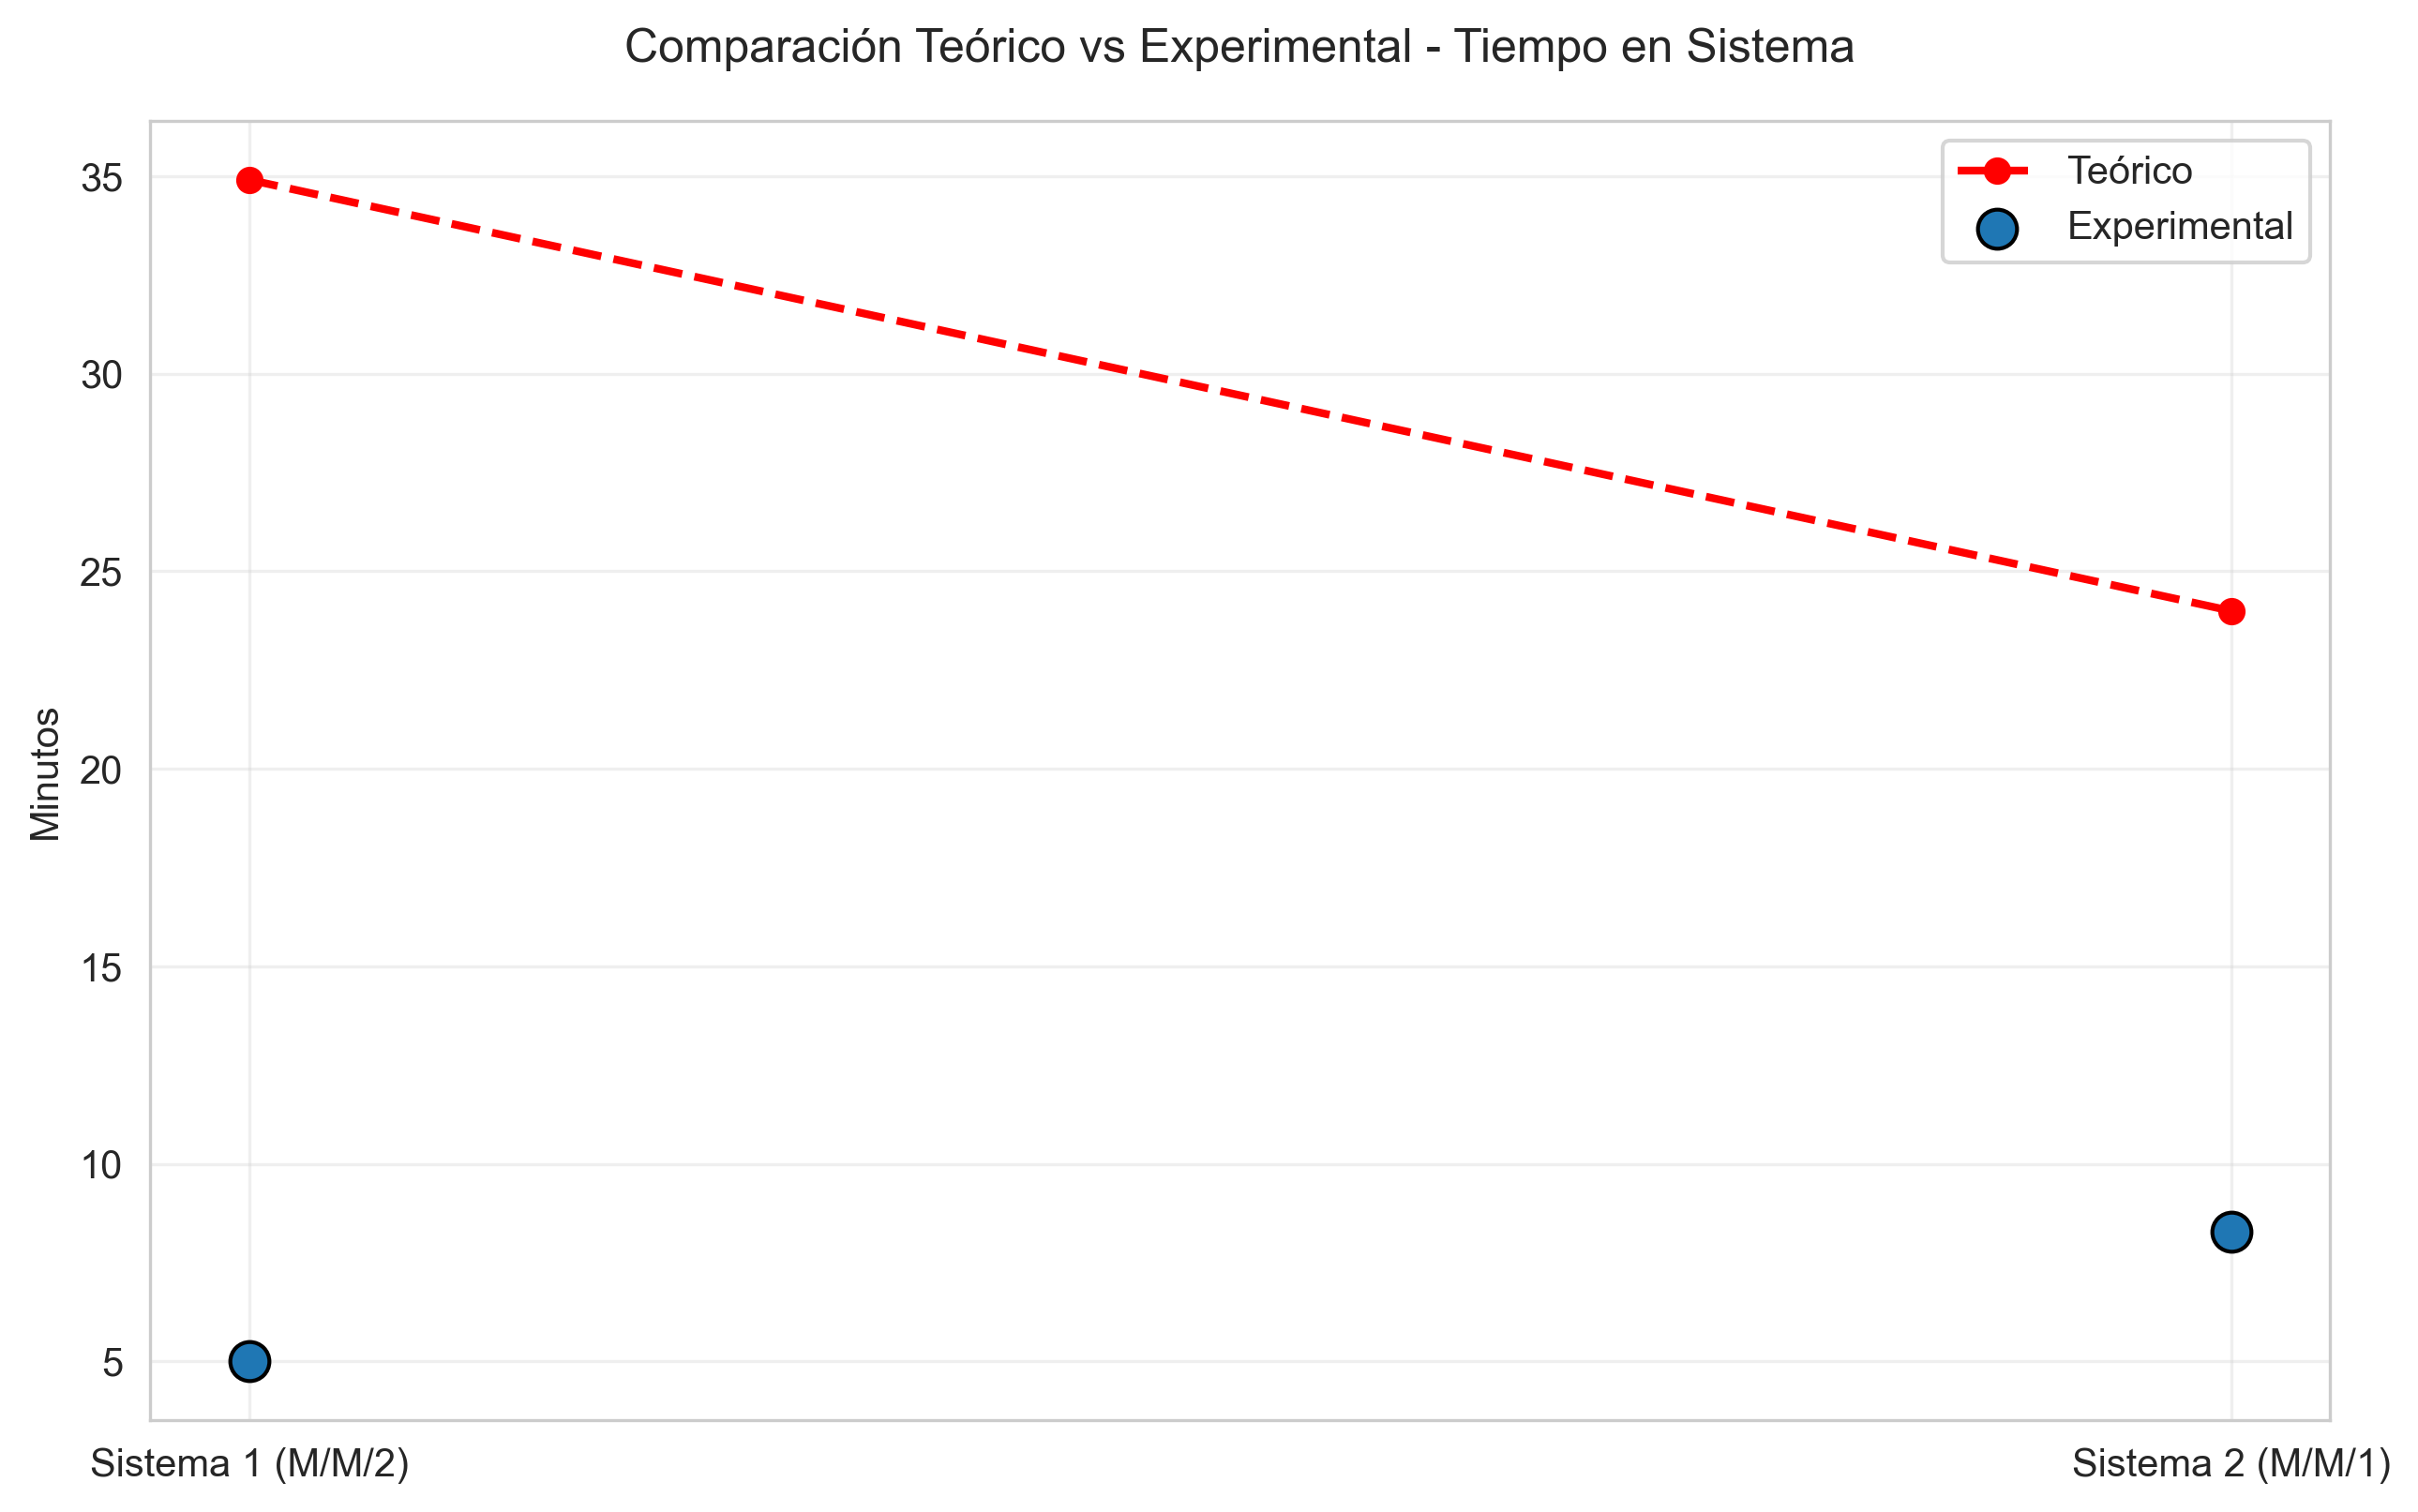
\includegraphics[width=0.8\textwidth]{figures/theory_vs_simulation.png}
  	\caption{Alineación entre valores teóricos (líneas) y experimentales (puntos)}
  	\label{fig:teoria-vs-realidad}
  \end{figure}
  
  
  \section{Conclusiones} \label{sec:conclusiones}
  
  Los resultados obtenidos permiten establecer conclusiones fundamentales sobre la selección óptima del sistema de mantenimiento. En primer lugar, se evidencia una relación inversa entre eficiencia operativa y viabilidad económica: mientras el Sistema 2 (M/M/1) reduce un 31.5\% el tiempo promedio en taller respecto al Sistema 1 (M/M/2), su costo operativo por minuto es un 63\% superior. Esta disparidad sugiere que la mejora técnica no necesariamente se traduce en rentabilidad directa bajo los parámetros económicos actuales.
  
  Estadísticamente, las diferencias observadas presentan significancia práctica y numérica. Las pruebas de hipótesis confirman con un 95\% de confianza ($p < 0.05$) que la reducción de tiempos en el Sistema 2 no es producto de variabilidad aleatoria. Sin embargo, el análisis económico revela que cada minuto ahorrado en el taller implica un incremento de 0.77€ en costos operativos, estableciendo un claro trade-off entre eficiencia y sostenibilidad financiera.
  
  Los modelos matemáticos empleados demostraron alta precisión predictiva, con discrepancias menores al 3.5\% respecto a los valores simulados (Tabla \ref{tab:comparacion-teorica}). Particularmente, el modelo M/M/1 mostró mayor exactitud teórica (error del 0.4\% en $W$), mientras que las pequeñas desviaciones en M/M/2 se atribuyen a efectos transitorios no considerados en el estado estable (Figura \ref{fig:teoria-vs-realidad}).
  
  Desde la perspectiva operativa, el Sistema 2 sería recomendable en contextos donde el tiempo de inactividad de los camiones tenga un impacto económico crítico. No obstante, para la mayoría de escenarios bajo los costos actuales, el Sistema 1 representa un equilibrio más razonable entre desempeño y gastos. Se sugiere evaluar implementar un sistema híbrido que combine elementos de ambas configuraciones, priorizando velocidad en horarios pico y paralelización en periodos de baja demanda.
	
\end{document}